\documentclass{beamer}
\input{../../packages.tex}
\input{../../slides_formatting.tex}

% Remove drop shadow by title
% https://tex.stackexchange.com/questions/3139/beamer-how-to-remove-shadow-under-the-title-on-a-given-frame
\setbeamertemplate{title page}[default][colsep=-4bp,rounded=true]

%gets rid of footer
%will override 'frame number' instruction above
%comment out to revert to previous/default definitions
\setbeamertemplate{footline}{}

%gets rid of bottom navigation symbols
\setbeamertemplate{navigation symbols}{}


\setbeamerfont*{frametitle}{family=\rmfamily, parent=structure}

%Information to be included in the title page:
\title{UFL + FEniCS: DSL Case Study}
\author{Russell Bentley}
\institute{
  Stony Brook University
}

\date{September 18 2025}

\begin{document}
\fontfamily{cmr}\selectfont

\frame{\titlepage}

%\placelogofalse
\begin{frame}{What are we talking about today?}
\begin{columns}
\column{0.58\linewidth}
\centering
\begin{outline}
  \1 Finite Element Method (FEM)
  \1 FEniCS 
  \1 Unified Form Language (UFL)
  \1 Discussion Questions (?)
\end{outline}

\column{0.38\linewidth}
\begin{center}
\centering
%\shadowimage[width=2.5cm]{example_1.png}
\shadowimage[width=\linewidth]{assets/fenics_logo.png}

% [trim={left bottom right top},clip]
%
\includegraphics[width=8.5cm, page=3, trim={0 9cm 14cm 0cm},clip]{assets/vec_db_figs.pdf}
\end{center}
\end{columns}
\end{frame}
%\placelogotrue


\placelogofalse
\begin{frame}{Finite Element Method (FEM)?}
\begin{columns}
\column{0.58\linewidth}
\centering
\begin{outline}
  \1 Family of numerical methods
  \2 Solve PDEs
  \2 Mathematical Modelling
  \2 Engineering / Science
  \1 History
  \2 Structural Mechanics in 1940s
  \2 NASTRAN in 1960s
  \2 Widely available now
  \1 Broad and well-funded
\end{outline}

\column{0.38\linewidth}
\centering

\begin{center}
\shadowimage[width=3.5cm]{assets/wiki_car_example.png} 

\shadowimage[width=2.0cm]{assets/fsi.png}
\shadowimage[width=2.0cm]{assets/BLAST_example.png}

\shadowimage[width=3.5cm]{assets/comsol.png}


\end{center}
\end{columns}
\blfootnote{Images from \href{https://en.wikipedia.org/wiki/Finite_element_method}{Wikipedia},
  \href{https://readfast.in/fluid-structure-interaction-in-fea-simulation/}{Readfast},
\href{https://computing.llnl.gov/projects/blast/triple-point-shock-interaction}{LNLL},
\href{https://www.comsol.com}{COMSOL}}
\end{frame}
\placelogotrue

\placelogofalse
\begin{frame}{Geometry and Meshing for FEM}
\begin{columns}
\column{0.58\linewidth}
\centering
\begin{outline}
  \1 FEM requires a discritazation 
  \1 Mesh of volumetric elements
  \1 Bottleneck in production
  \1 Massive research topic
  \1 Meshing Out-of-scope for today 
  \1 Return to meshes later
\end{outline}

\column{0.38\linewidth}
\begin{center}
\centering
%\shadowimage[width=2.5cm]{example_1.png}

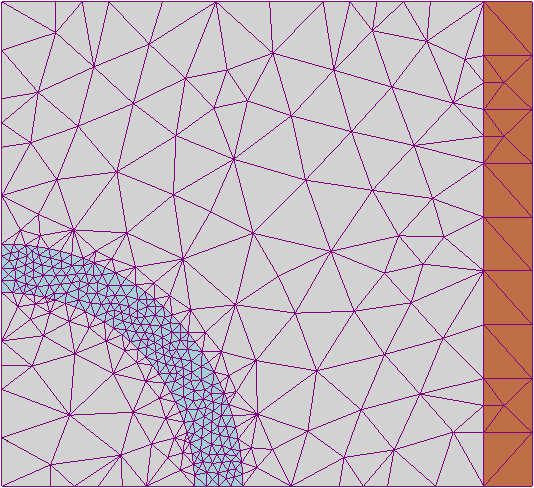
\includegraphics[width=2.8cm]{assets/Example_of_2D_mesh.png}

\vspace{0.2cm}

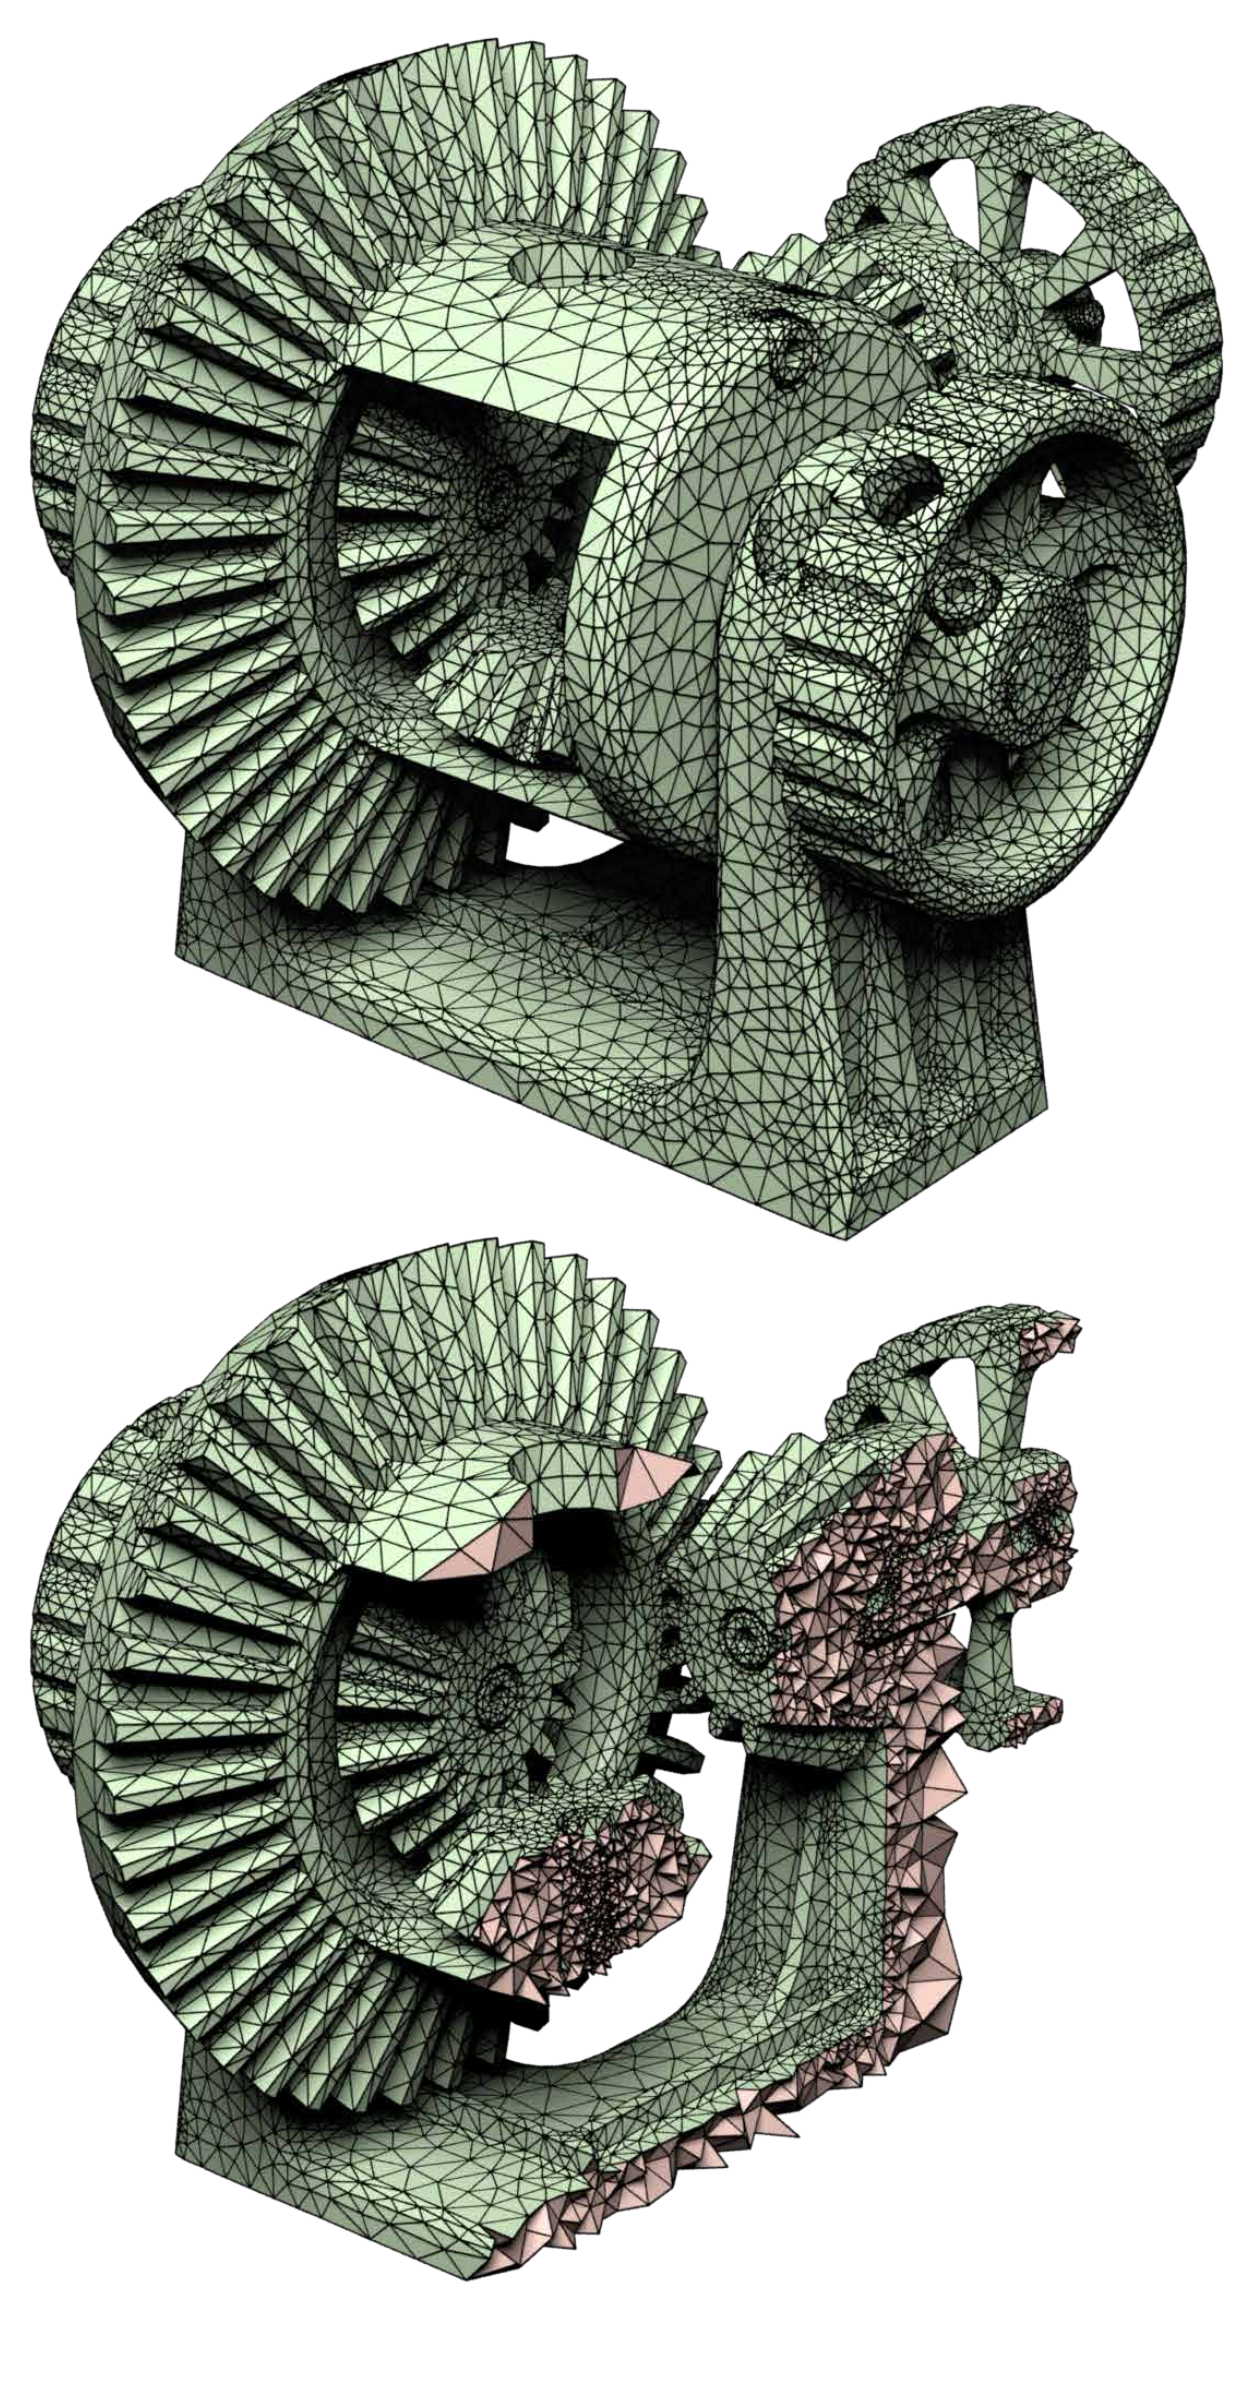
\includegraphics[width=2.5cm]{assets/mesh_example_01.png}


% [trim={left bottom right top},clip]
%
\includegraphics[width=8.5cm, page=3, trim={0 9cm 14cm 0cm},clip]{assets/vec_db_figs.pdf}
\end{center}
\end{columns}
\blfootnote{Images from \href{https://upload.wikimedia.org/wikipedia/commons/8/80/Example_of_2D_mesh.png}{Wikipedia},
\href{https://github.com/wildmeshing/fTetWild}{fTetWild}}
\end{frame}
\placelogotrue



\placelogofalse
\begin{frame}{Basis Functions: FEM Solution Structure}
\begin{columns}
\column{0.58\linewidth}

  $$
    -\Delta u = f \text{ in } \Omega
  $$

\begin{outline}
  \1 Approximate continuous solution to strong form
  \1 Construct solution peicewise
  \2 Basis functions live on element nodes
  \2 Overlap in the elements
  \1 Solution is are weights for basis functions
  \1 Interpolation over mesh for solution
\end{outline}

\column{0.38\linewidth}
\begin{center}
\centering
%\shadowimage[width=2.5cm]{example_1.png}
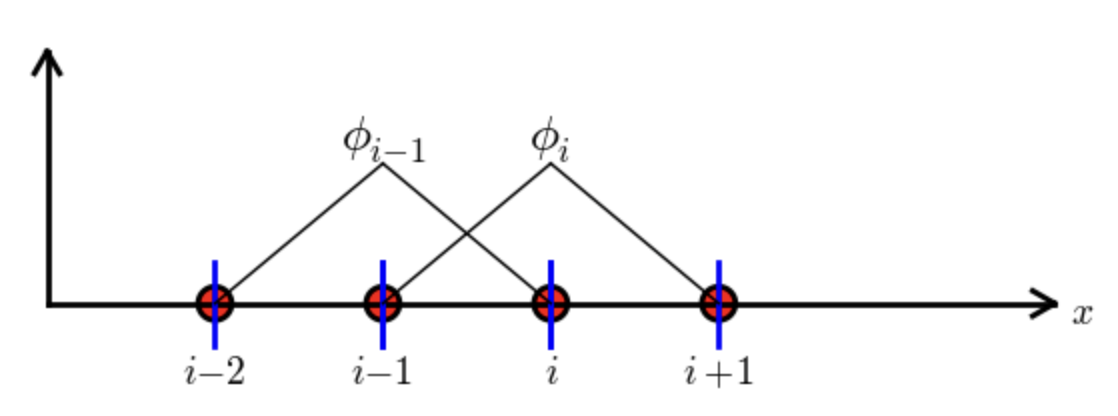
\includegraphics[width=\linewidth]{assets/hat_basis.png}

\vspace{0.5cm}

\shadowimage[width=\linewidth]{assets/base_functions_overlap.png}

% [trim={left bottom right top},clip]
%
\includegraphics[width=8.5cm, page=3, trim={0 9cm 14cm 0cm},clip]{assets/vec_db_figs.pdf}
\end{center}
\end{columns}
\end{frame}
\placelogotrue


\begin{frame}{FEM: Weak Formulation}
  \begin{columns}
  \column{0.56\linewidth}

  \begin{outline}
    \1 Derive solution from trial function space
    \1 Requiring equality everywhere is impossible
    \1 Relaxed continuity restrictions
    \1 Assert that residual (error) is orthogonal to \textit{test function } space
    \1 Usually use $\phi_i$ from mesh
  \end{outline}

  \vspace{0.2cm}

  \textit{Strong Form:} $ L(u) = f \text{ on } \Omega$

  \vspace{0.2cm}

  \textit{Variational Form:} $ \int_{\Omega} (L(u) - f)v = 0$

  \column{0.30\linewidth}

  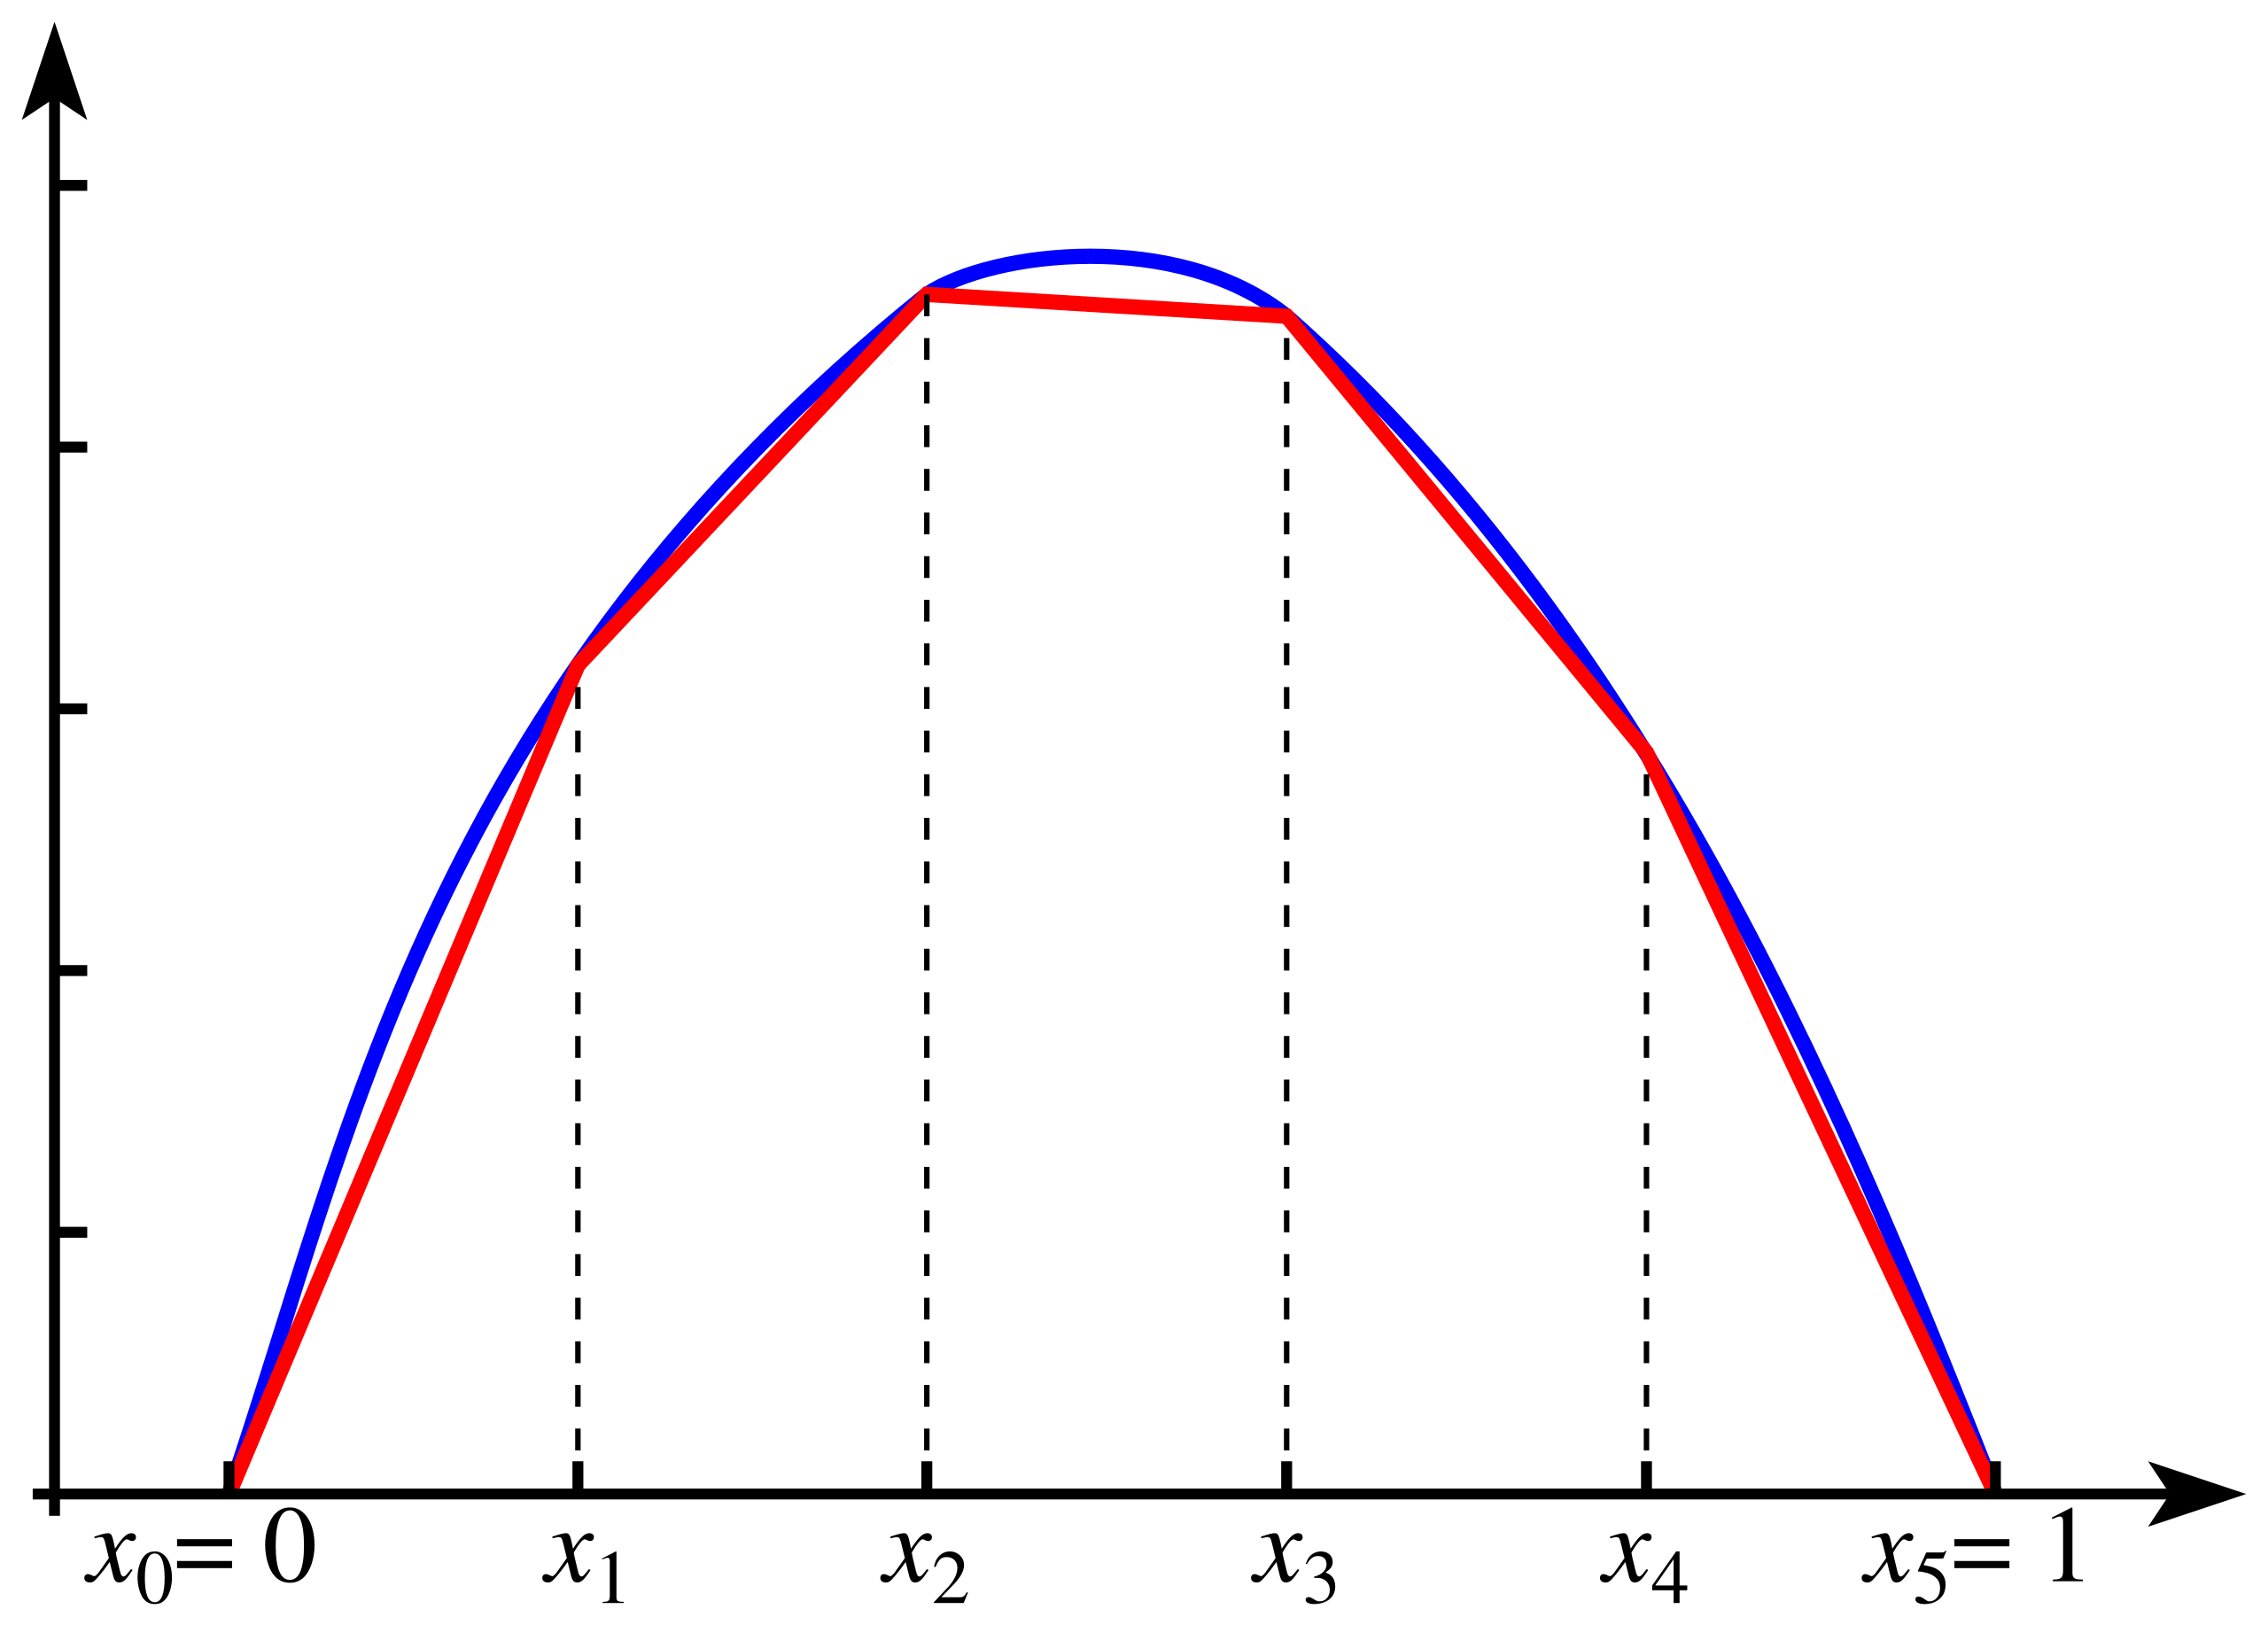
\includegraphics[width=\linewidth]{assets/fem_approx.png}

\end{columns}
\end{frame}




%\placelogofalse
\begin{frame}{The FEniCS Project}
\begin{columns}
\column{0.58\linewidth}
\centering
\begin{outline}
  \1 Collection of opensource software 
  \1 Used to create models with FEM
  \1 Origins in 2002
  \1 Steady development / rewrites
  \1 Very popular for research
  \1 Unified Form Language (UFL) 
\end{outline}

\column{0.38\linewidth}
\begin{center}
\centering

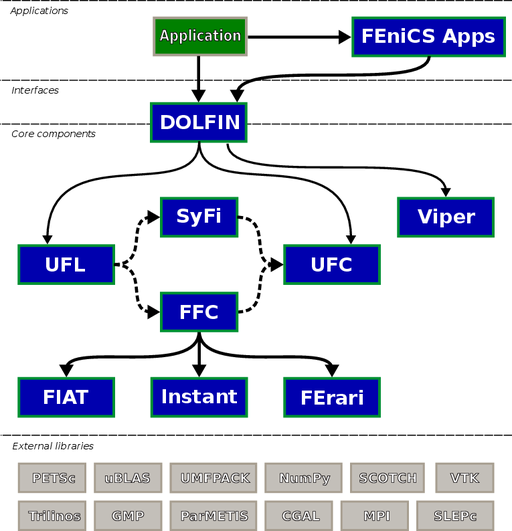
\includegraphics[width=\linewidth]{assets/Fenics-map.png}

%\shadowimage[width=2.5cm]{example_1.png}

%\includegraphics[width=2.5cm]{example_3.png}

% [trim={left bottom right top},clip]
%
\includegraphics[width=8.5cm, page=3, trim={0 9cm 14cm 0cm},clip]{assets/vec_db_figs.pdf}
\end{center}
\end{columns}
%\blfootnote{From \href{https://en.wikipedia.org/wiki/FEniCS_Project#/media/File:Fenics-map.png}{Wikipedia}}
\end{frame}
%\placelogotrue


%\placelogofalse
\begin{frame}{Unified Form Language (UFL)}
\begin{columns}
\column{0.58\linewidth}
\centering
\begin{outline}
  \1 Introduced in 2013
  \2 Grew out of FEniCS Form Compiler (FCC)
  \1 DSEL in Python
  \1 Writing equations
  \2 Variational Forms
  \2 Suitable to solve with FEM
  \2 Syntax closely matches notation
  \1 Adopted by other projects
\end{outline}

\column{0.38\linewidth}
\begin{center}
\centering
\lstinline{a = c * dx + e * ds}

\vspace{0.2cm}

represents

$$a = \int_{\Omega} c \ dx + \int_{\partial \Omega} e \ ds$$
\end{center}
\end{columns}
\end{frame}
%\placelogotrue


\placelogofalse
\begin{frame}{Poisson's Equation: Hello World of PDEs}
\begin{columns}
\column{0.58\linewidth}
  $$
    -\nabla^2 u = -\Delta u = f \text{ in } \Omega
  $$

\begin{outline}
  \1 Constain Divergence of Gradient
  \1 Ubiquitous 
  \2 Thermal Equilibrium
  \2 Electrostatics
  \2 Gravitational Potential
  \2 Vector Graphics Shading
  \2 Component of larger problems
  \1 Solve for $u$
\end{outline}


\column{0.38\linewidth}
\begin{center}
\centering
%\shadowimage[width=2.5cm]{example_1.png}

%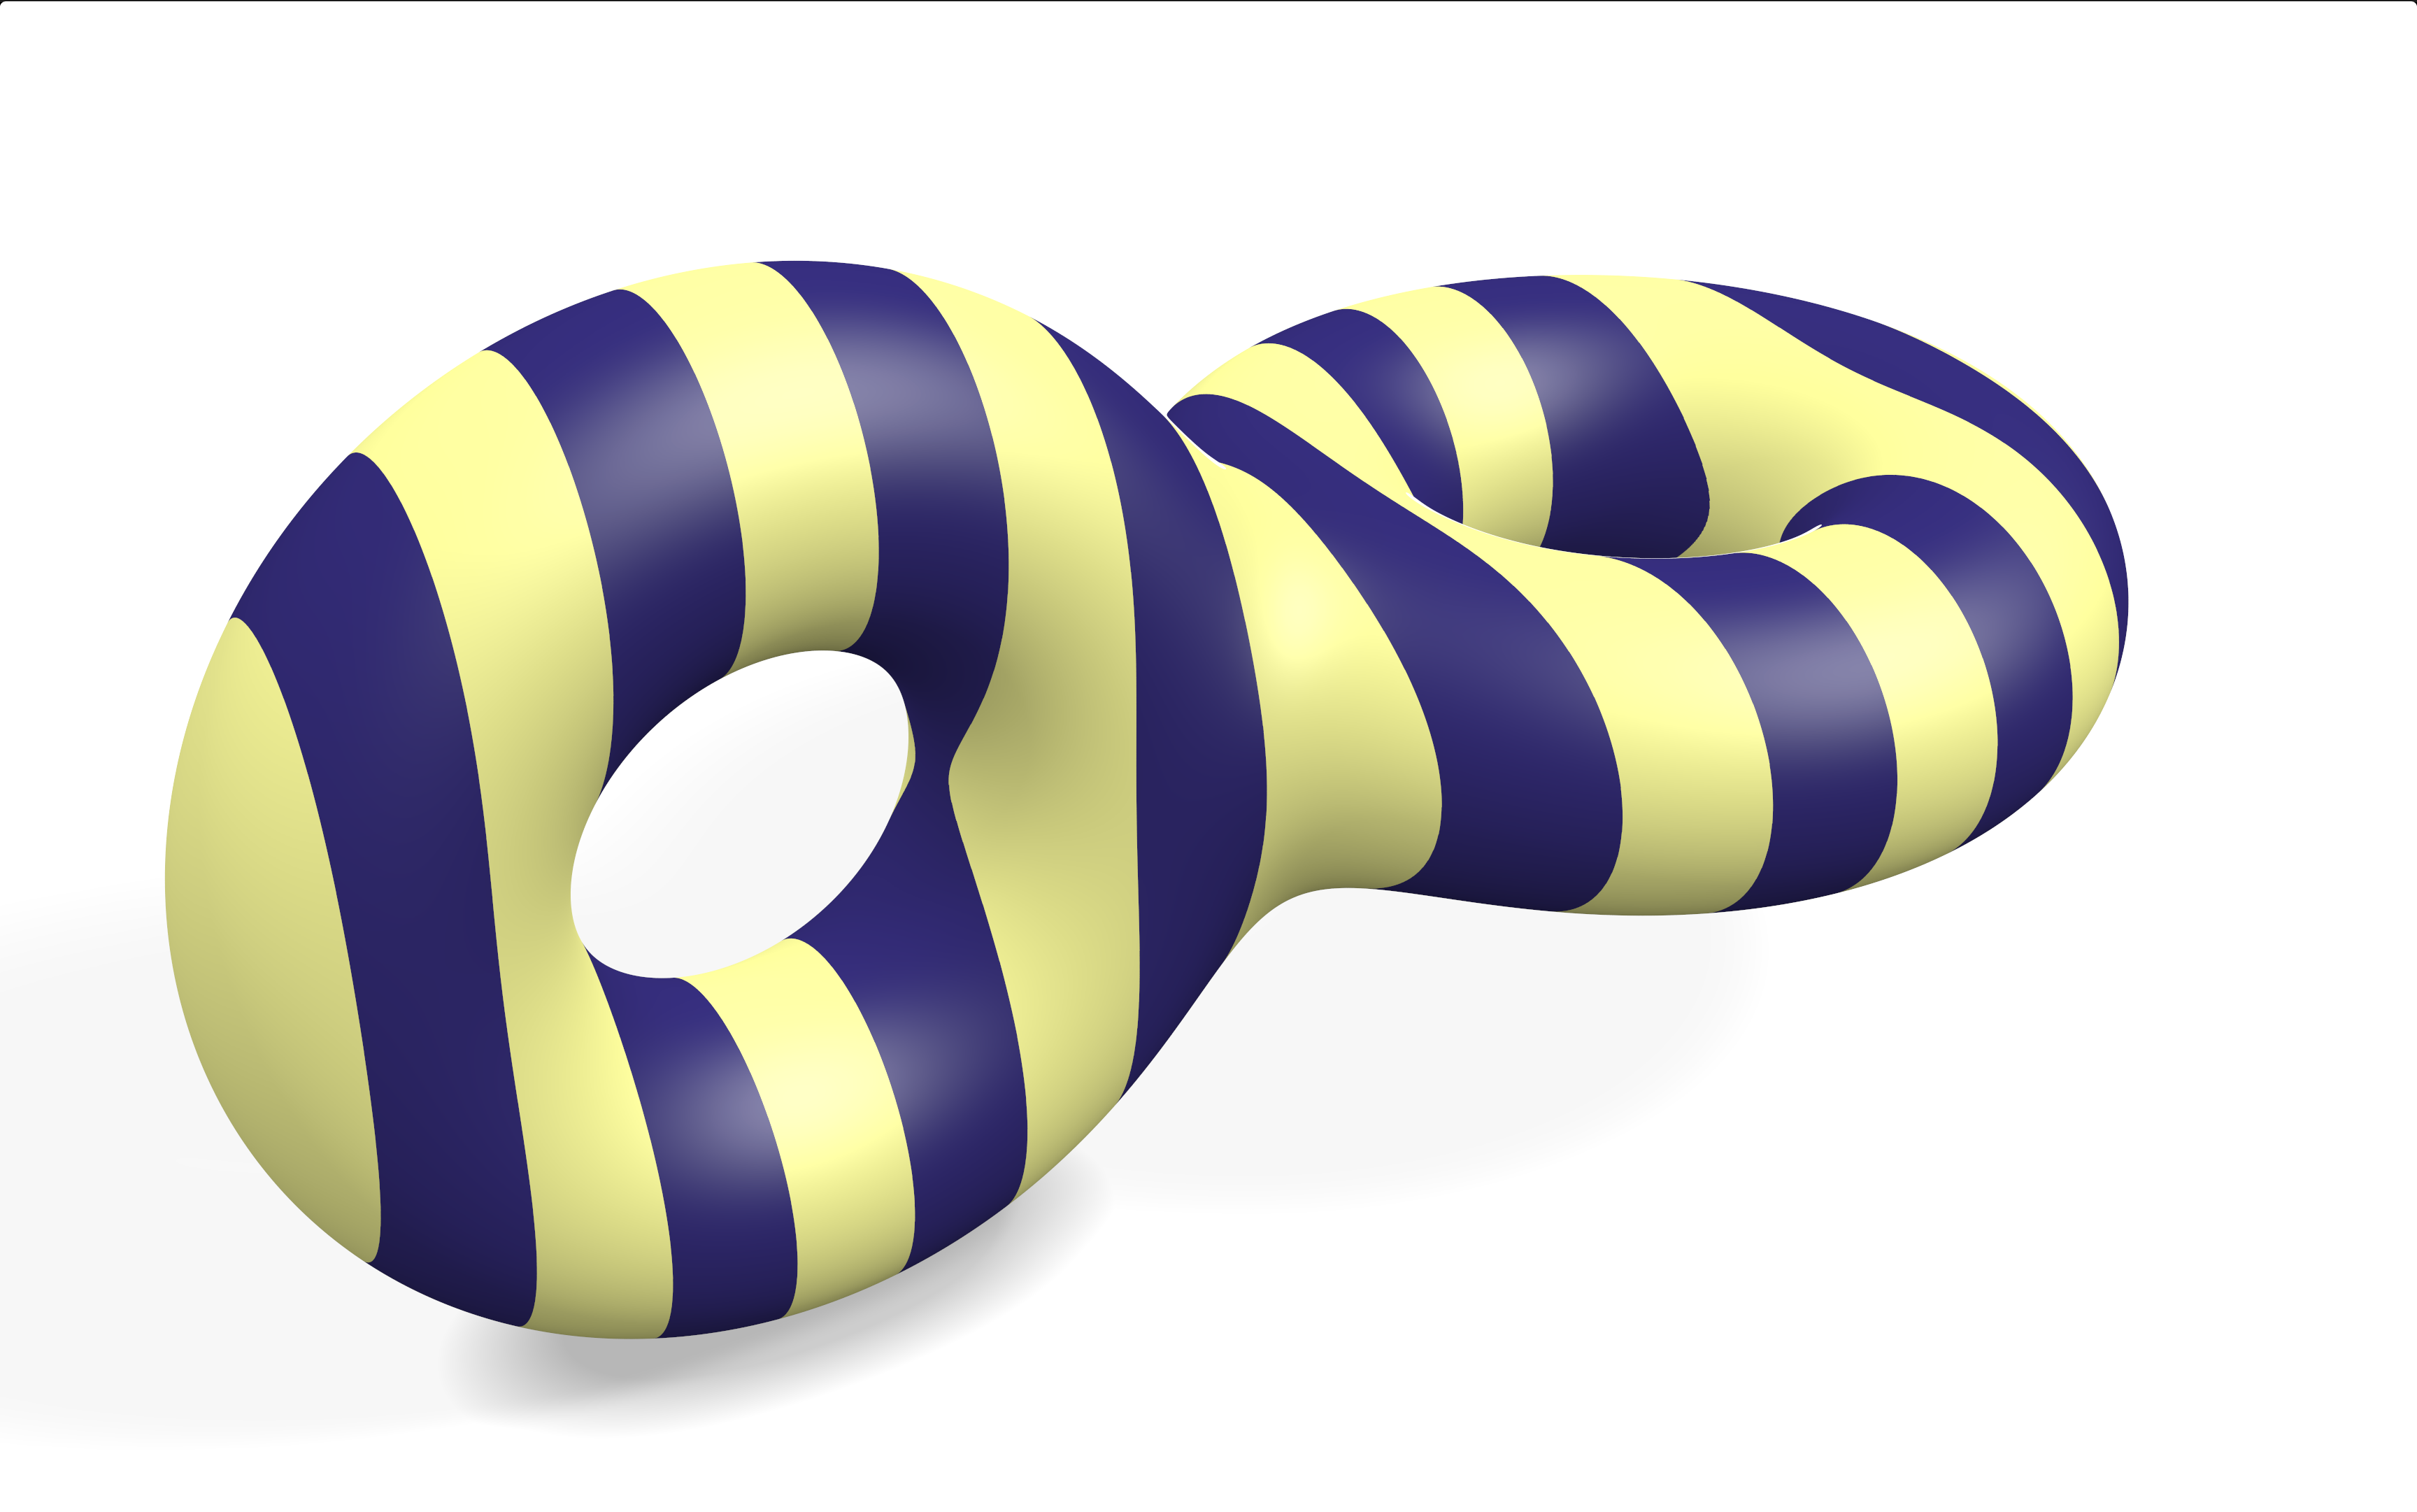
\includegraphics[width=4cm, trim{0 0 0 0.2cm}, clip]{assets/poisson_1.png}
\shadowimage[width=\linewidth, trim={0 0 0 0.1cm}, clip]{assets/poisson_1.png}

\vspace{0.2cm}

\shadowimage[width=\linewidth, trim={0 0 0 0.1cm}, clip]{assets/poisson_2.png}

%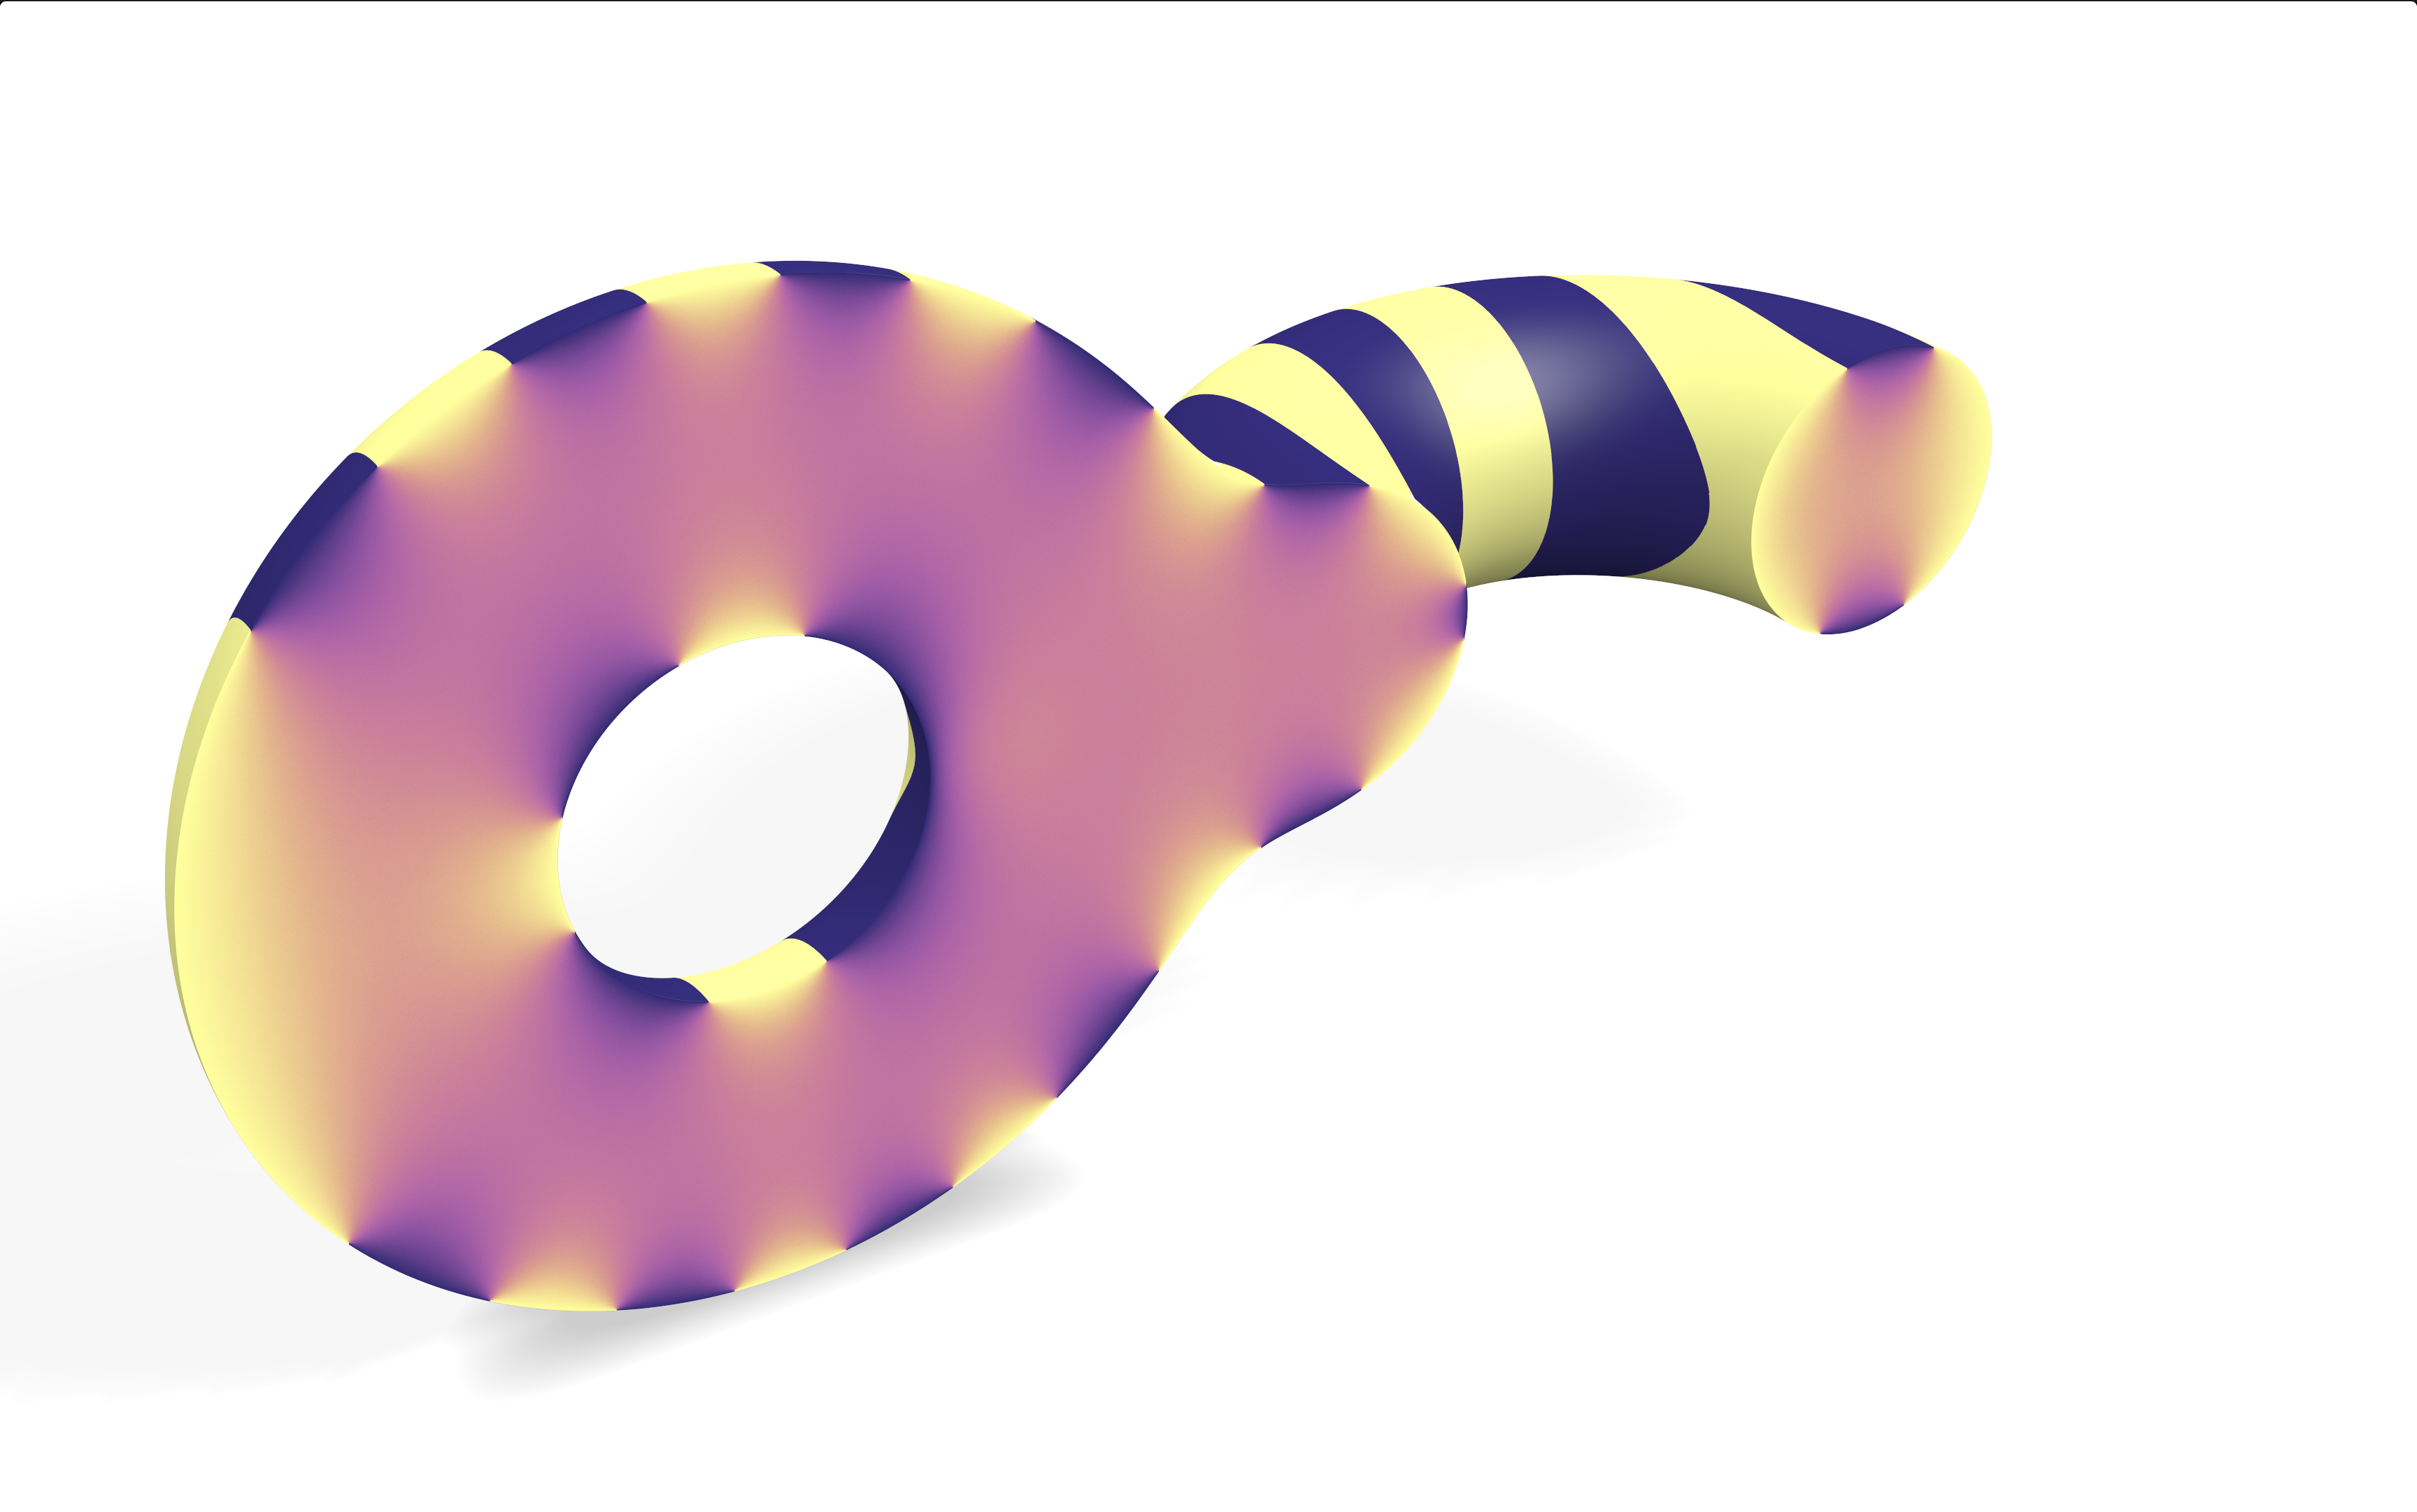
\includegraphics[width=4cm, trim{0 0 0 0.2cm}, clip]{assets/poisson_2.png}


% [trim={left bottom right top},clip]
%
\includegraphics[width=8.5cm, page=3, trim={0 9cm 14cm 0cm},clip]{assets/vec_db_figs.pdf}
\end{center}
\end{columns}
\end{frame}
\placelogotrue


\begin{frame}{Variational Form for Poisson's Equation}
$$
- \Delta u = f \text{ in } \Omega
$$

Multiply both sides by a \textit{test function} $v$

Integrate over the domain $\Omega$

$$
\int_{\Omega}(-\Delta u) v \ dx = \int_{\Omega} f v \ dx
$$

Apply integration by parts, test function disappears on the boundary.

$$
\int_{\Omega} \nabla u \cdot \nabla v dx = \int_{\Omega} f v \ dx
$$


\textit{Variational Form}
Find $u \in V$ such that

$$
a(u, v) = L(v) \ \forall v \in \hat{V},
$$
\end{frame}
%\placelogotrue

\begin{frame}[fragile]{Variational Form for Poisson's Equation in UFL}
\begin{lstlisting}[language=Python]
from ufl import *

# Mesh and function space 
# Provided by higher-level FEniCS code
V = FunctionSpace(mesh, "Lagrange", 1)

u = TrialFunction(V)   # unknown
v = TestFunction(V)    # test function
f = Function(V)        # source term

a = dot(grad(u), grad(v)) * dx
L = f * v * dx
\end{lstlisting}
\end{frame}




\begin{frame}{Poisson's Equation: The Discrete Problem}
Solution is weighted sum of basis functions
$$
  u(x) = \sum^N_{j = 1} U_j \phi_j(x)
$$
Variational Form becomes
$$
  \sum^N_{j = 1} U_j \int_{\Omega} \nabla \phi_j \cdot \nabla \hat{\phi}_i \ dx = \int_{\Omega} f \hat{\phi}_i \ dx \ i = 1, 2, \cdots, N
$$
Compute $U$ by solving linear system $AU = b$, where
\begin{align*}
A_{ij} &= \int_{\Omega} \nabla \phi_j \cdot \nabla \hat{\phi}_i \ dx \\
b_i &= \int_{\Omega} f \hat{\phi}_i \ dx
\end{align*}
\end{frame}

\placelogofalse
\begin{frame}{Global Assembly and Linear Solve}
\begin{columns}
\column{0.58\linewidth}
\begin{align*}
  A_{ij} &= \int_{\Omega} \nabla \phi_j \cdot \nabla \hat{\phi}_i \ dx \\
         &= \sum_{\{E\}} \int_{\Omega_E} \nabla \phi_j \cdot \nabla \hat{\phi}_i \ dx
\end{align*}

\begin{outline}
  \1 $A_{ij}$ is non-zero when $\phi_i$ and $\phi_j$ share an element
  \1 $A$ matrix is sparse
  \1 Use a sparse linear solver
\end{outline}

\column{0.38\linewidth}
\centering
\begin{center}
%\shadowimage[width=2.5cm]{example_1.png}

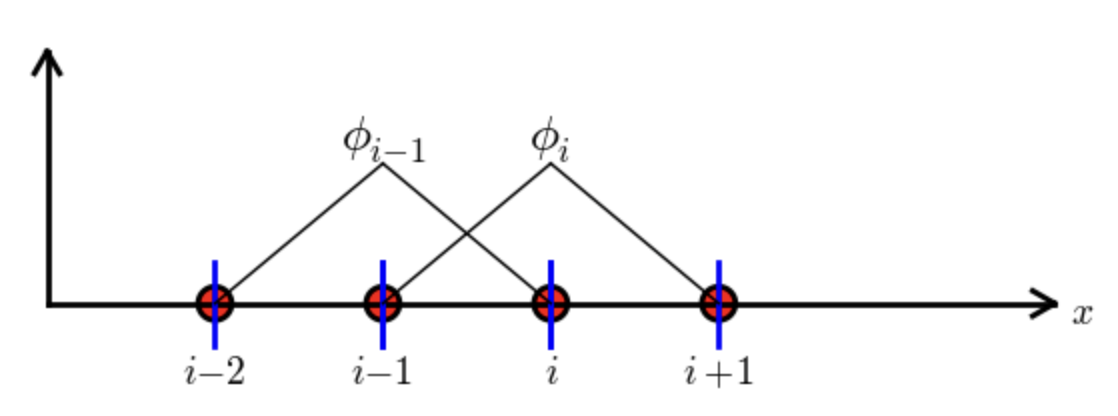
\includegraphics[width=\linewidth]{assets/hat_basis.png}


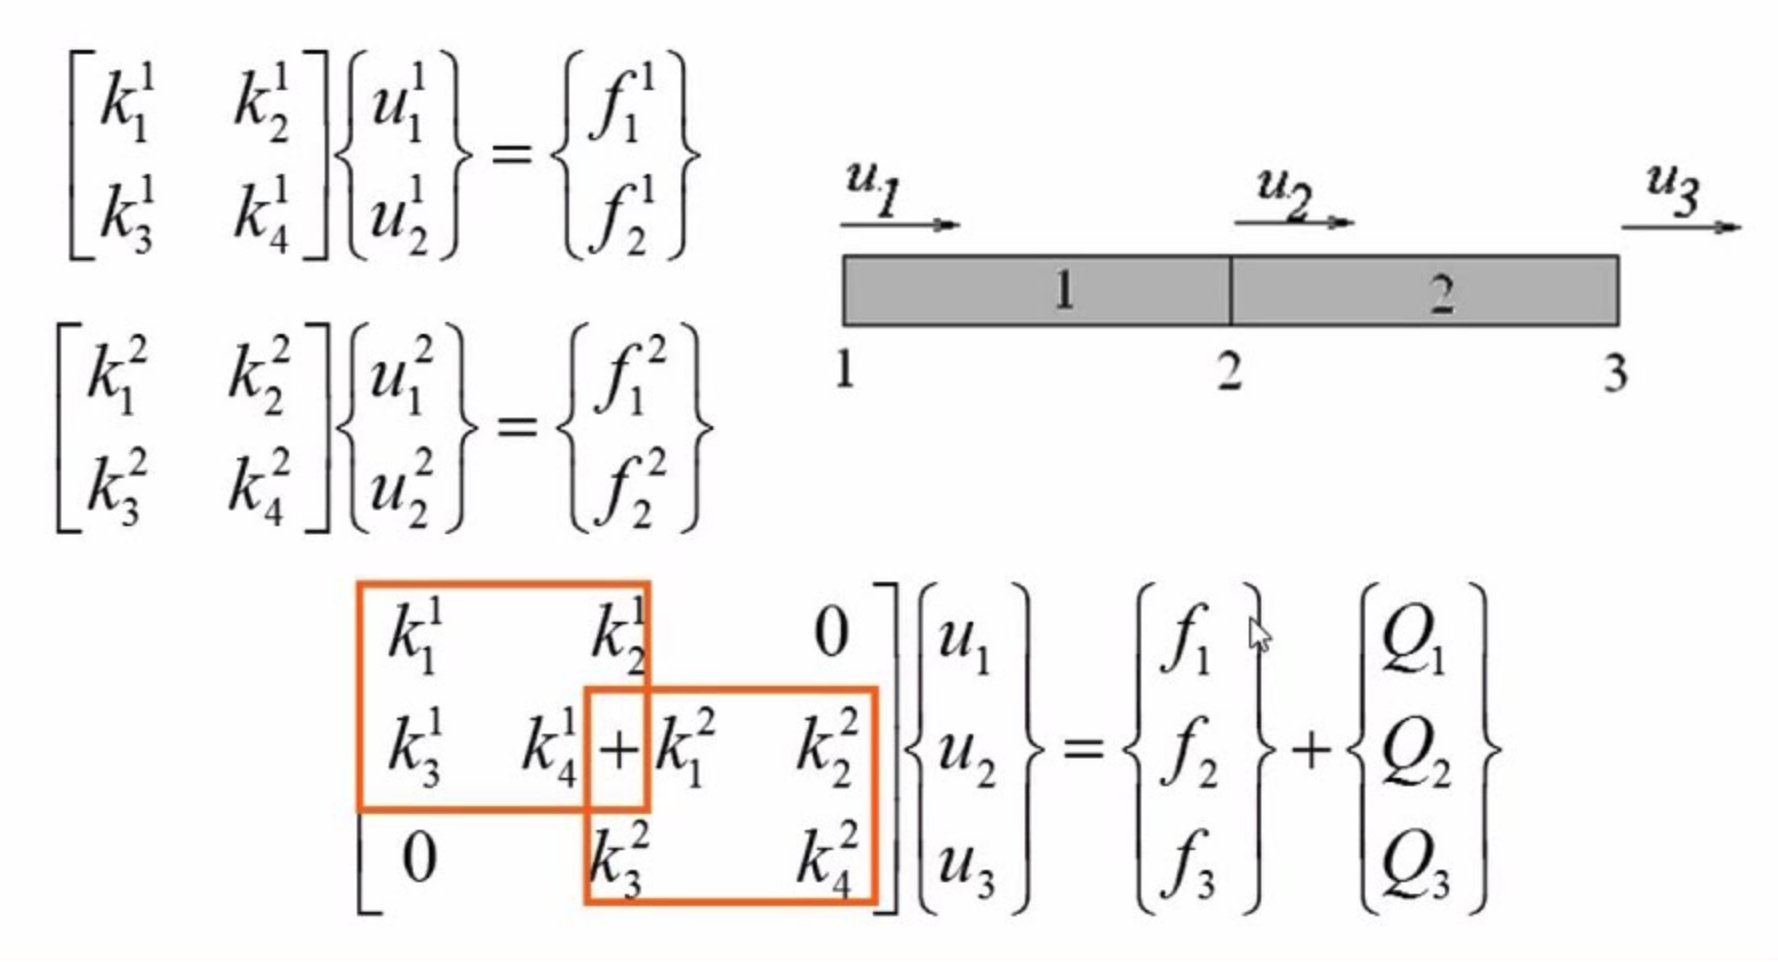
\includegraphics[width=3.5cm]{assets/two_element_example.png}

\vspace{0.2cm}

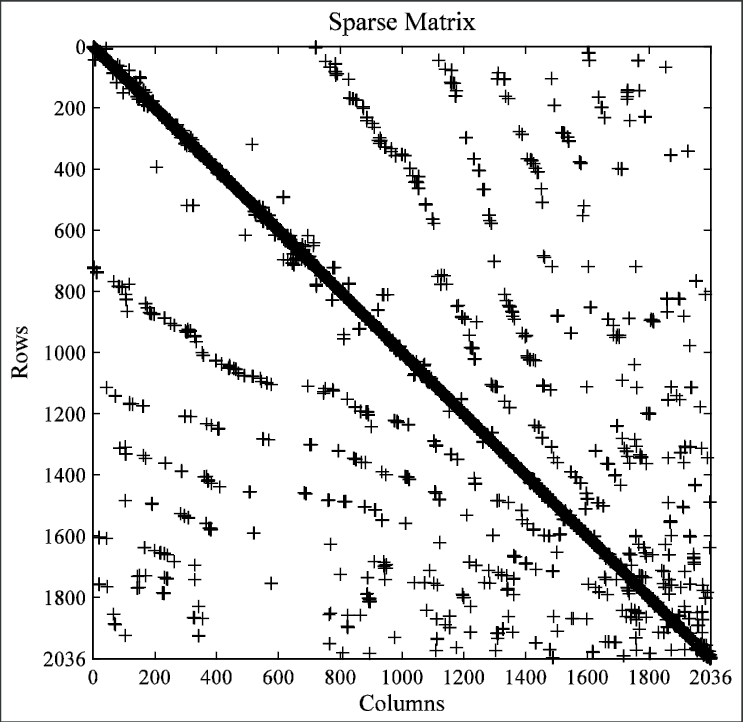
\includegraphics[width=3.5cm]{assets/sparsity_pattern.png}


% [trim={left bottom right top},clip]
%
\includegraphics[width=8.5cm, page=3, trim={0 9cm 14cm 0cm},clip]{assets/vec_db_figs.pdf}
\end{center}
\end{columns}
\end{frame}
\placelogotrue

\begin{frame}{Integrating with Quadrature}
  \begin{columns}
\column{0.58\linewidth}
\begin{outline}
  \1 Integrals mean quadrature rules 
  \2 $\left\{(w_k \in \mathbb{R}, x_k \in \Omega)\right\}$ such that $\sum_{k = 1}^{K} w_k = 1$
  \1 Integrators have nested structure 
  \2 For each element
  \2 For each basis pair
  \2 For each quadrature point
\end{outline}

\begin{align*}
A_{ij} &= \int_{\Omega_E} \nabla \phi_j \cdot \nabla \hat{\phi}_i \ dx \\
       &\approx \sum_{k = 1}^{K} w_k \nabla \phi_j(x_k) \cdot \nabla \hat{\phi}_i (x_k)
\end{align*}


\column{0.38\linewidth}
\centering
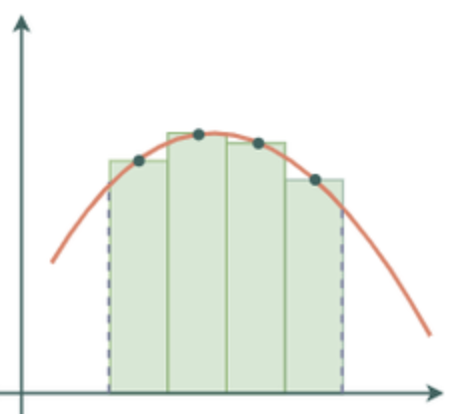
\includegraphics[width=3.5cm]{assets/midpoint.png}
\end{columns}
\end{frame}




\placelogofalse
\begin{frame}{Coding FEM by Hand}
\centering
\begin{center}
\shadowimage[width=9.0cm]{assets/intact_integrator.png}
\end{center}
\end{frame}
\placelogotrue


\placelogofalse
\begin{frame}{Unified Form Language (UFL)}
\begin{columns}
\column{0.48\linewidth}
\centering
\begin{outline}
\1 \textit{Focused} on multilinear forms
\2 Linear in argument spaces $\left\{ V_j \right\}_{j = 1}^{\rho}$
\2 Parameterized by coefficent spaces $\left\{ W_k \right\}_{k = 1}^{n}$
$$a: W_1 \times \cdot \times W_n \times V_1 \times \cdot \times V_{\rho} \rightarrow \mathbb{R}$$
\1 Expression based 
\2 Terminals and operators
\2 Tensor shape as type 
\end{outline}

\column{0.48\linewidth}
\begin{center}
\centering
%\shadowimage[width=2.5cm]{example_1.png}

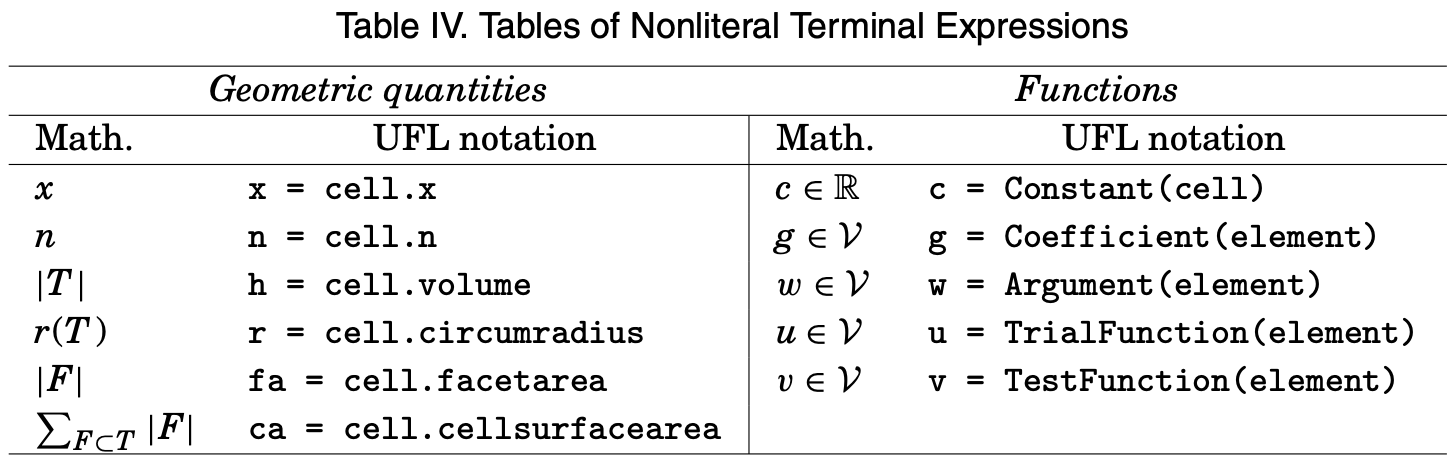
\includegraphics[width=4cm]{assets/literals.png}

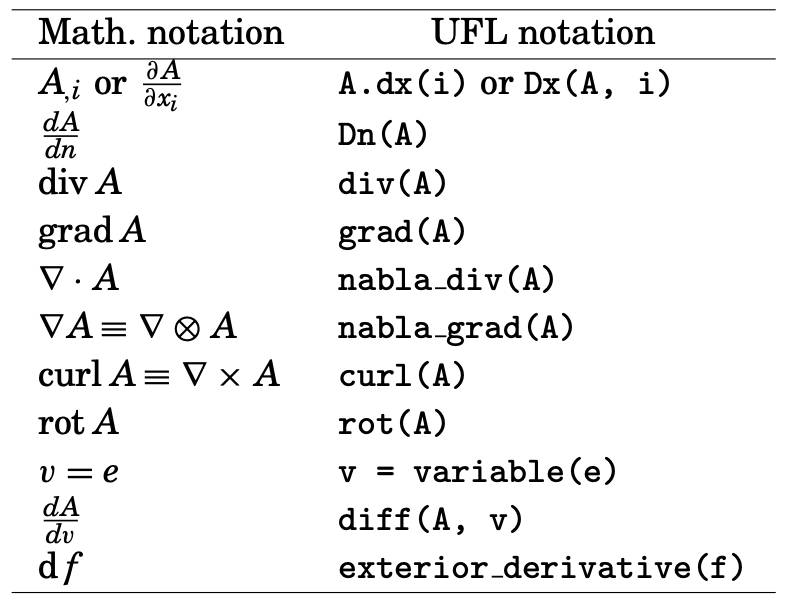
\includegraphics[width=2.3cm]{assets/ops.png}

\vspace{0.2cm}

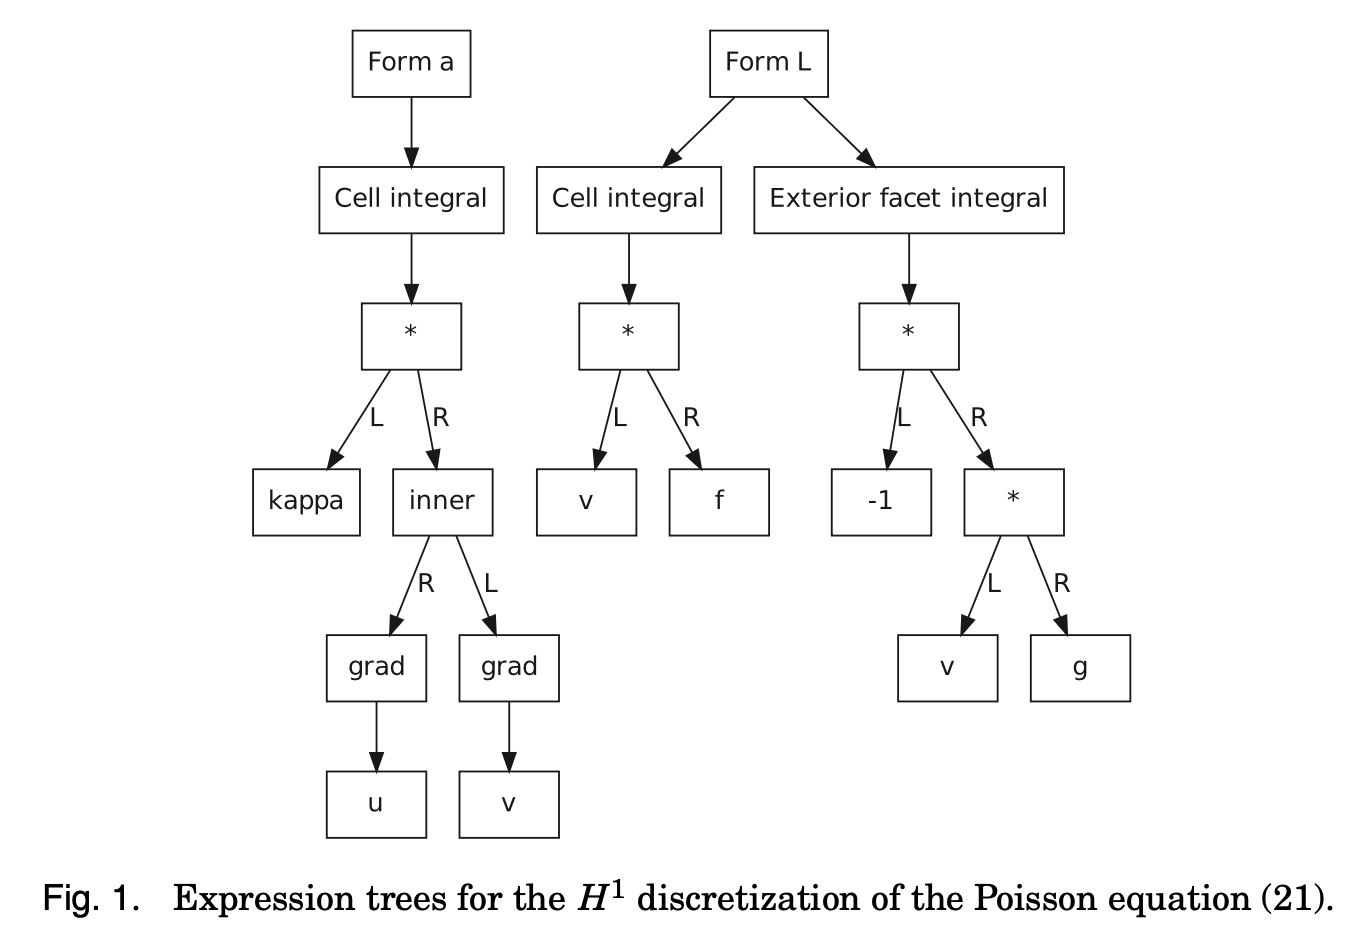
\includegraphics[width=4.5cm]{assets/trees.png}


% [trim={left bottom right top},clip]
%
\includegraphics[width=8.5cm, page=3, trim={0 9cm 14cm 0cm},clip]{assets/vec_db_figs.pdf}
\end{center}
\end{columns}
\end{frame}
\placelogotrue


%\placelogofalse
\begin{frame}{UFL Applications}
\begin{columns}
\column{0.58\linewidth}
\centering
\begin{outline}
  \1 Write your equations in math-like notation
  \1 Get an efficient solver
  \1 General purpose
  \2 Cardiac modeling
  \2 Plasma Physics
  \2 Fracture Mechanics
  \2 Differentiable Physics
  \2 Parameter Estimation
  \2 Optimization
\end{outline}

\column{0.38\linewidth}
\begin{center}
\centering
%\shadowimage[width=2.5cm]{example_1.png}

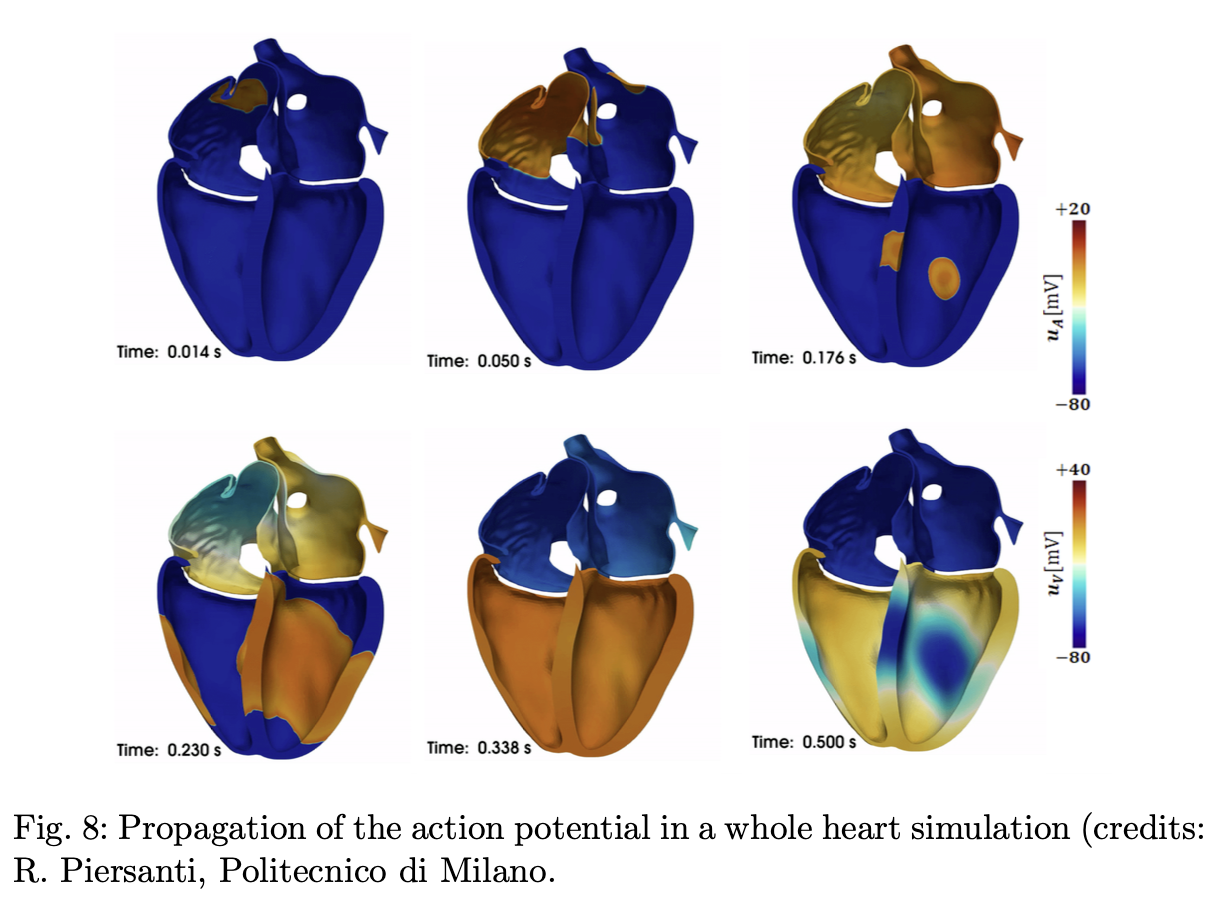
\includegraphics[width=4.5cm]{assets/cardiac.png}

\vspace{0.2cm}

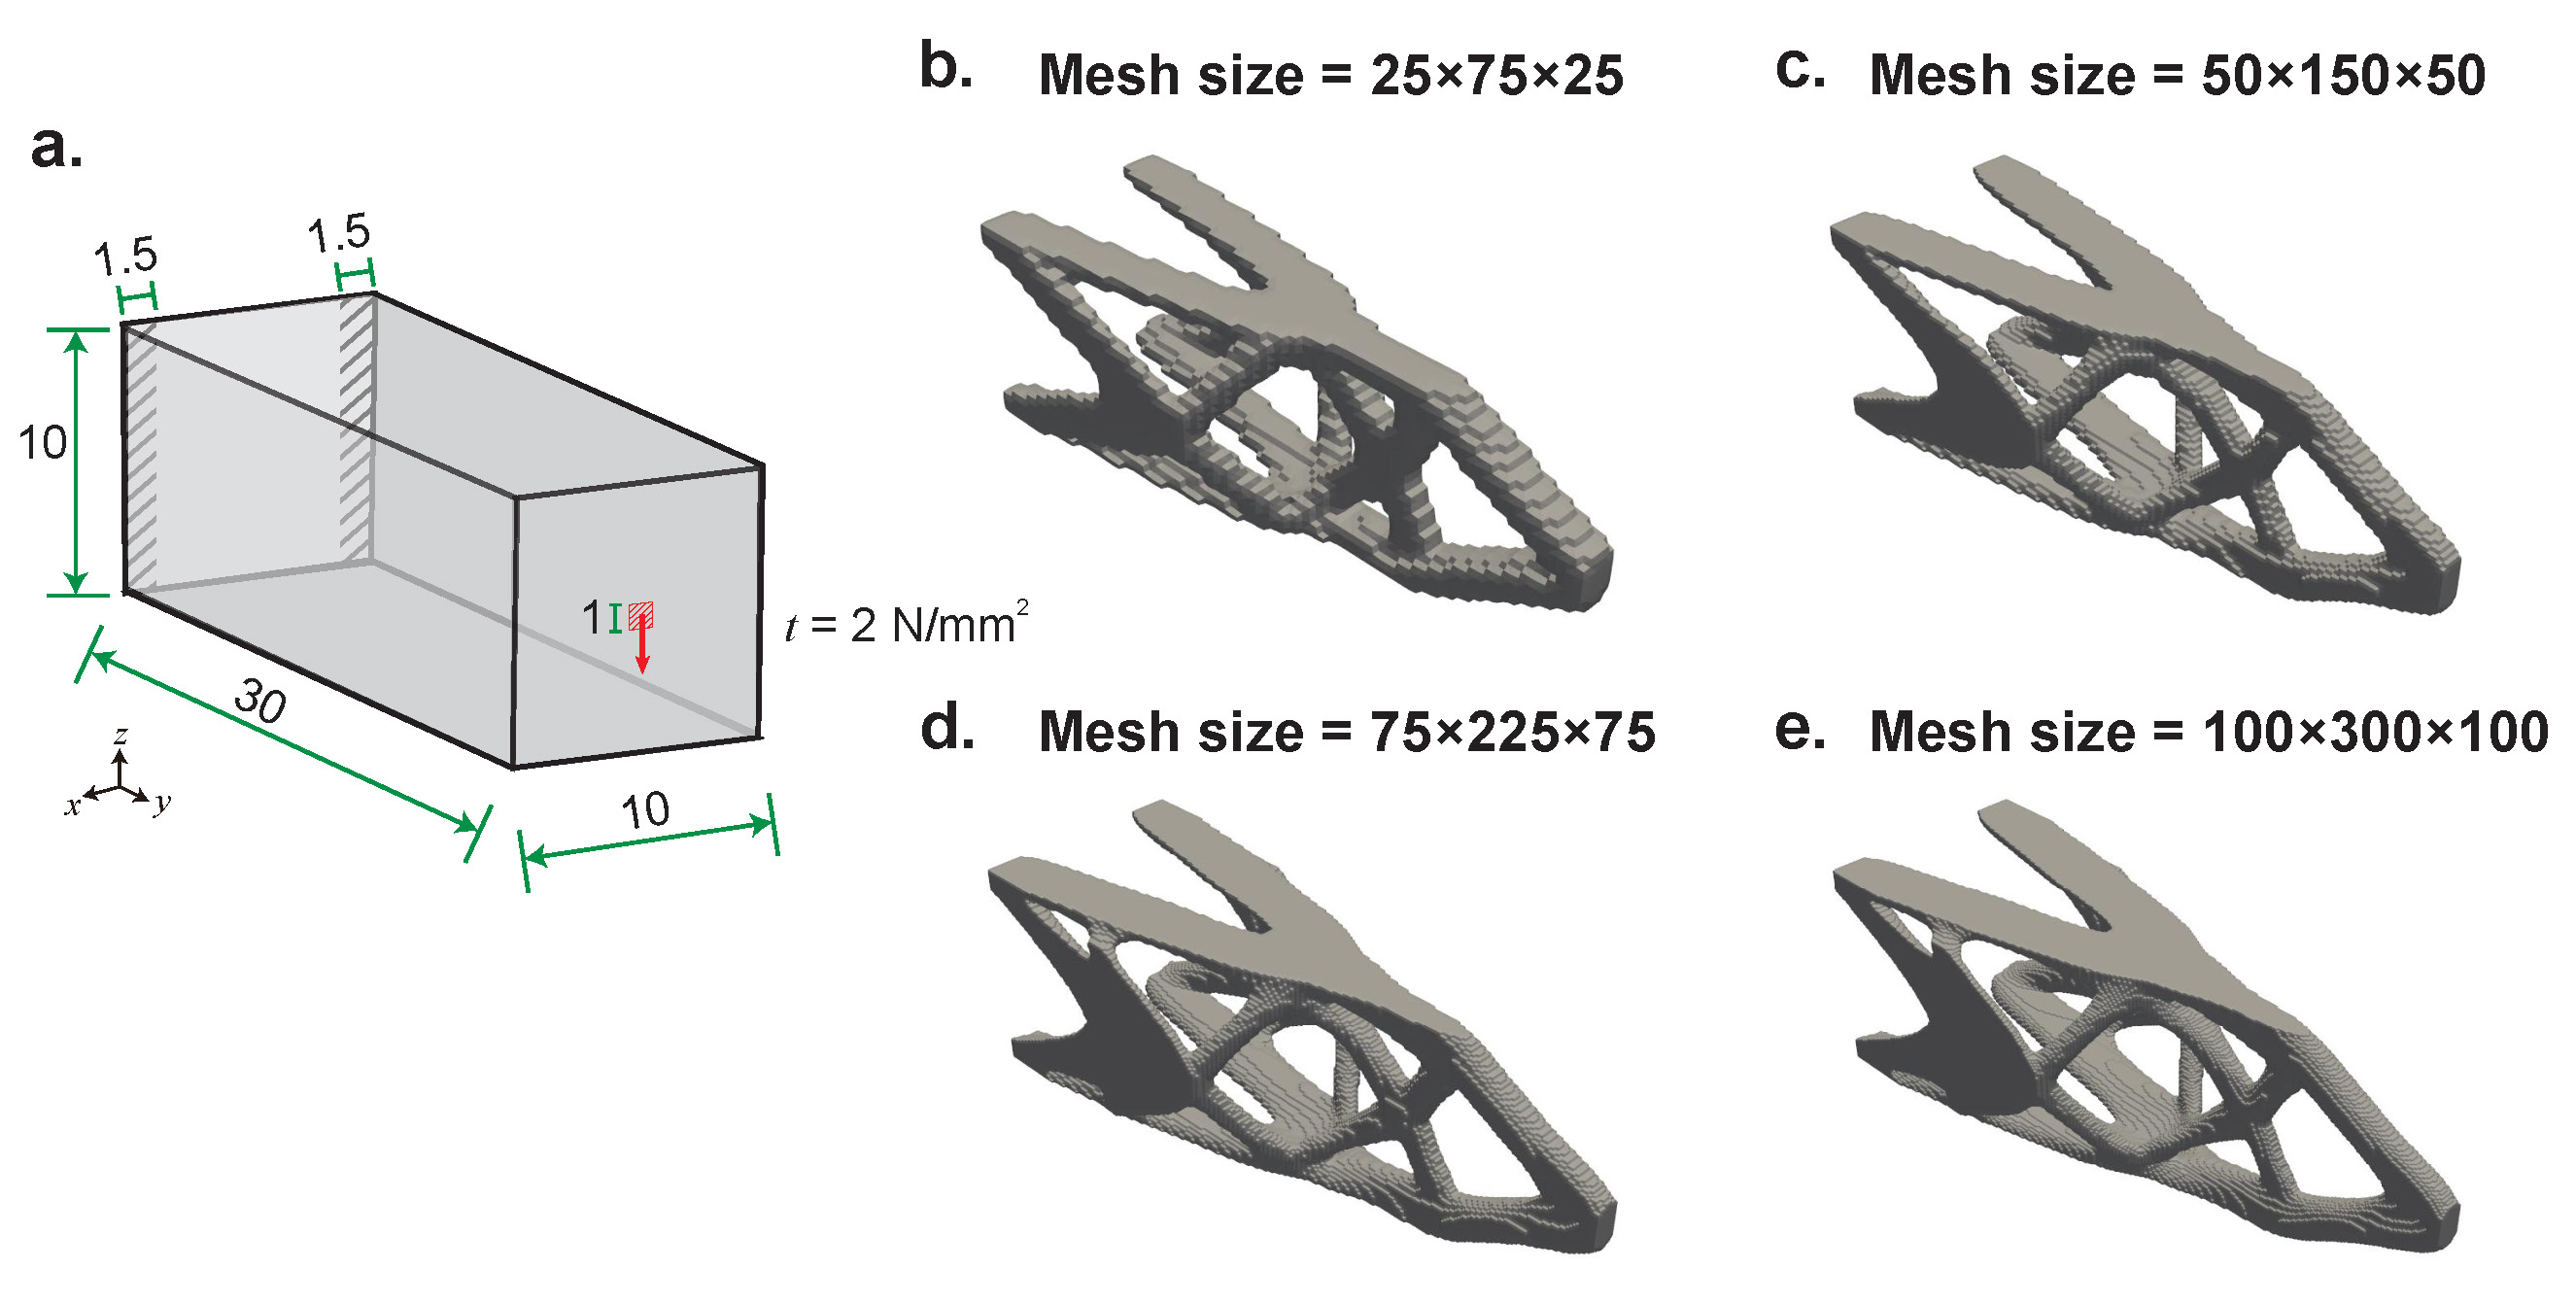
\includegraphics[width=4.5cm]{assets/beam_3d.jpg}


% [trim={left bottom right top},clip]
%
\includegraphics[width=8.5cm, page=3, trim={0 9cm 14cm 0cm},clip]{assets/vec_db_figs.pdf}
\end{center}
\end{columns}
\end{frame}
%\placelogotrue


%%\placelogofalse
\begin{frame}{Poisson's Equation}
\begin{columns}
\column{0.58\linewidth}
$$ - \Delta u = f \text{ in } \Omega, u = f(x, y, z) \text{ on } \nabla \Omega
$$

Multiply both sides by a \textit{test function} $v$

Integrate over the domain $\Omega$

$$
\int_{\Omega}(-Delta u) v \ dx = \int_{\Omega} f v \ dx
$$

Apply integration by parts to move derivatives off of $u$ , such that $u \in H^1$, not $C^2$.

$$
\int_{\Omega} \nabla u \cdot \nabla v dx = \int_{\Omega} f v \ dx
$$


\textit{Variation Form}
Find $u \in V$ such that

$$
a(u, v) = L(v) \ \forall v \in V,
$$
Where
\begin{align*}
  a(u, v) &= \int_{\Omega} \nabla u \cdot v \ dx \text{ Bilinear form} \\
  L(v) &= \int_{\Omega} f  \ dx \text{ Linear Form}
\end{align*}

\column{0.38\linewidth}
\begin{center}
\centering
%\shadowimage[width=2.5cm]{example_1.png}

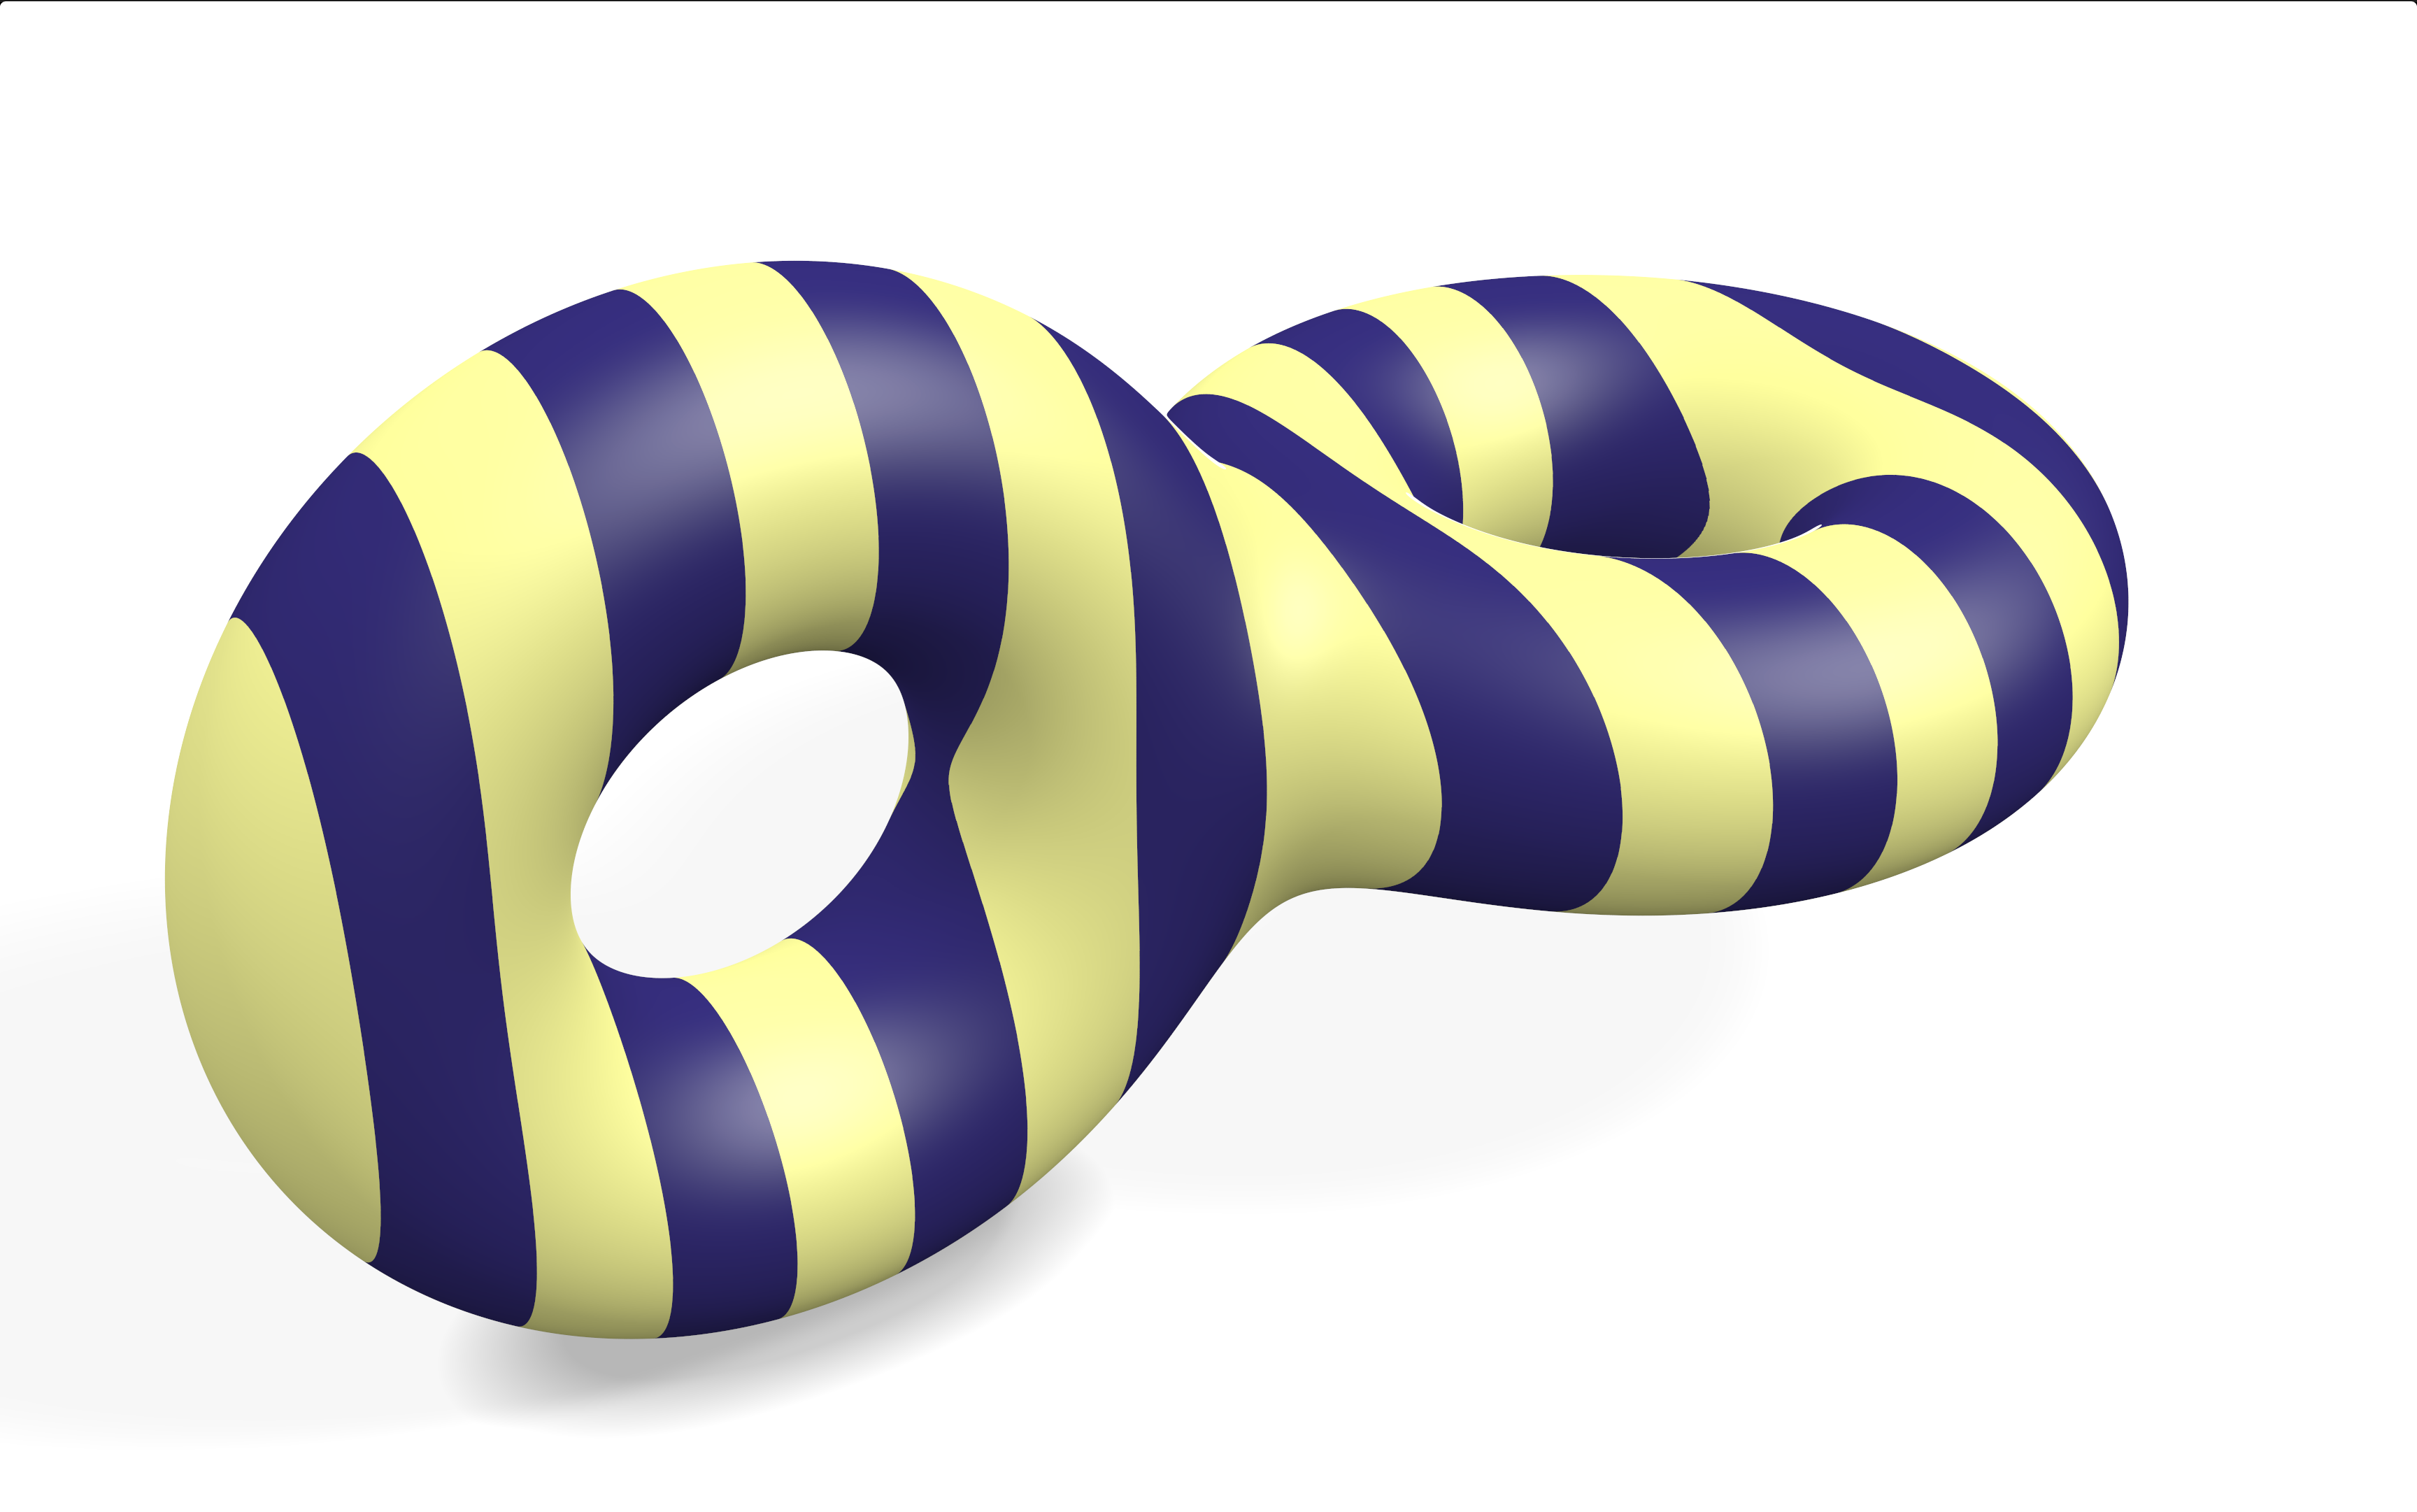
\includegraphics[width=2.5cm]{assets/poisson_1.png}

\vspace{0.2cm}

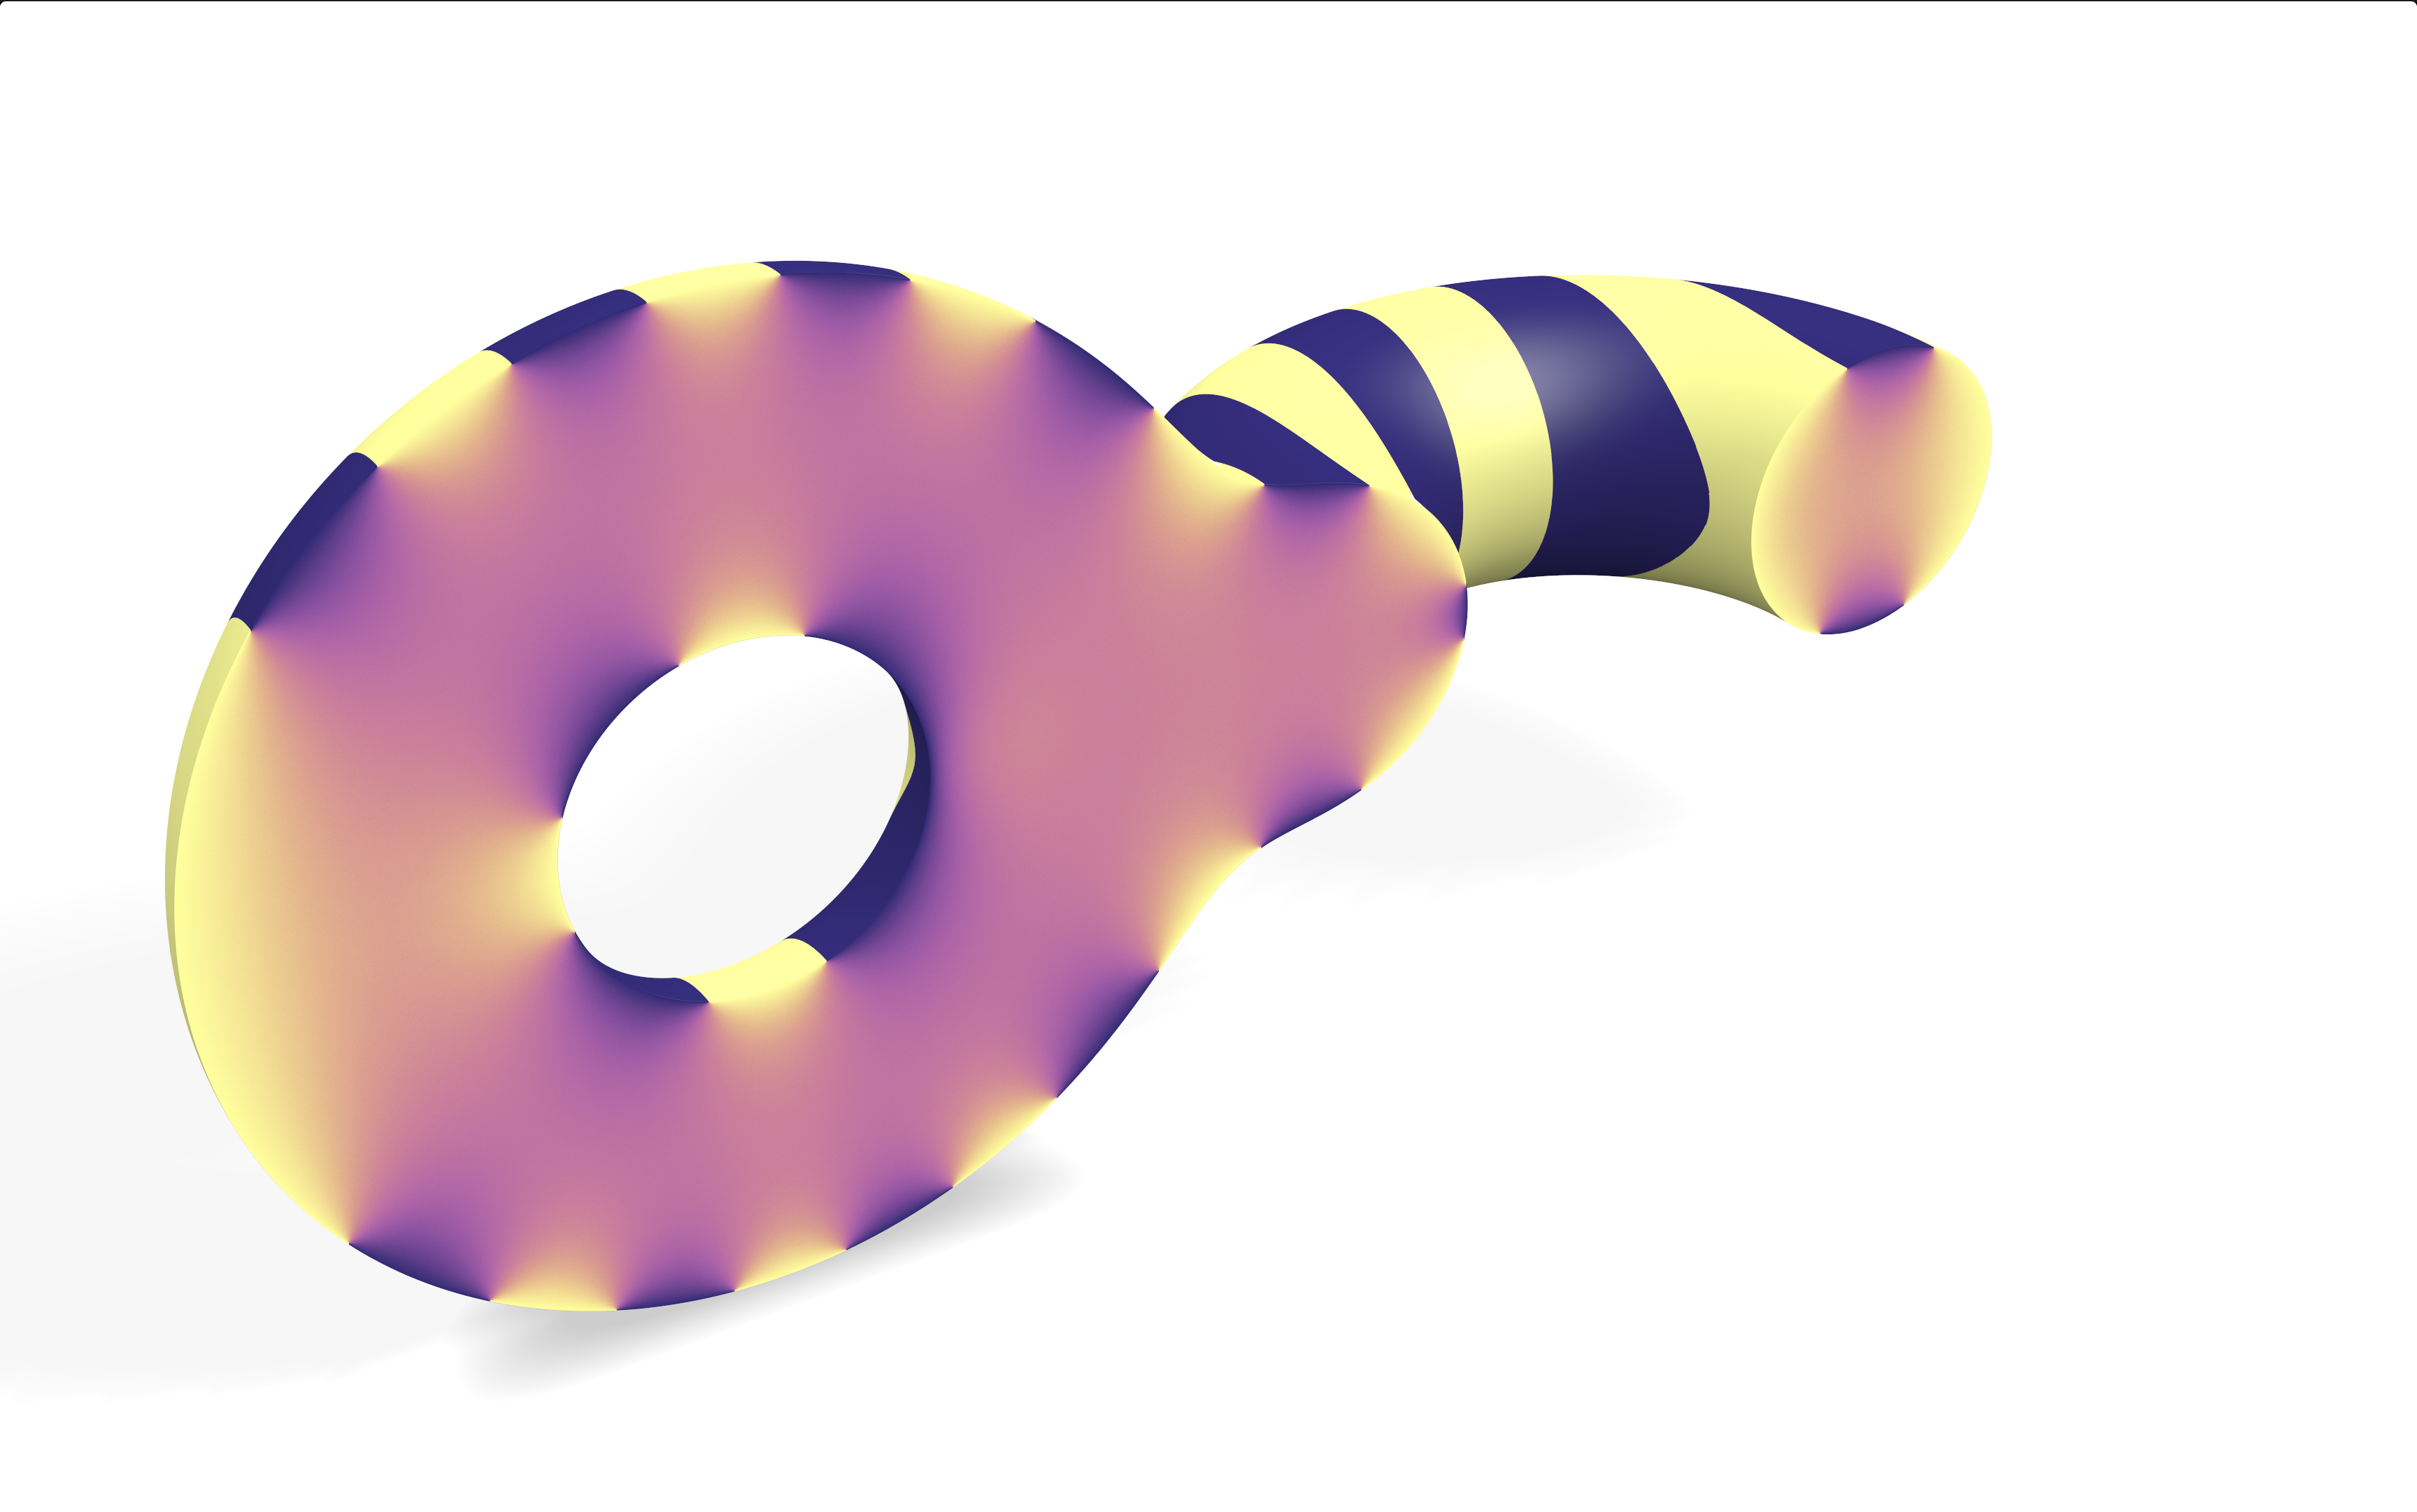
\includegraphics[width=2.5cm]{assets/poisson_2.png}


% [trim={left bottom right top},clip]
%
\includegraphics[width=8.5cm, page=3, trim={0 9cm 14cm 0cm},clip]{assets/vec_db_figs.pdf}
\end{center}
\end{columns}
\end{frame}
%\placelogotrue

\begin{frame}[fragile]{Python Example}
\begin{lstlisting}[language=Python]
from ufl import *

# Mesh and function space (provided by higher-level FEniCS code, not UFL itself)
V = FunctionSpace(mesh, "Lagrange", 1)

u = TrialFunction(V)   # unknown
v = TestFunction(V)    # test function
f = Function(V)        # source term

a = dot(grad(u), grad(v)) * dx
L = f * v * dx
\end{lstlisting}
\end{frame}

%\placelogofalse
\begin{frame}{Poisson Problem: Finite Element Discritization Pt1}
  \begin{align*}
    -\Delta u &= f \text{ in } \Omega \\
    -\Delta u v &= f v \text { in } \Omega \\
    \int_{\Omega} \nabla u \cdot \nabla v \ dx
    - \int_{\partial \Omega} \partial_n u v \ ds 
                &= \int_{\Omega} f v \ dx \\
   \int_{\Omega} \nabla u \cdot \nabla v \ dx
                &= \int_{\Omega} f v \ dx 
                - \int_{\Gamma_N} g v \ ds \ \forall v \in \hat{V}\\
  \end{align*}
\end{frame}
%\placelogotrue

\begin{frame}{Poisson Problem: Finite Element Discritization Pt2}
  \begin{align*}
    u_h(x) &= \sum^N_{j = 1} U_j \phi_j(x) \\
    \sum^N_{j = 1} U_j \int_{\Omega} \nabla \phi_j \cdot \nabla \hat{\phi}_i \ dx &= \int_{\Omega} f \hat{\phi}_i \ dx - \int_{\Gamma_N} g \hat{\phi}_i \ ds \ i = 1, 2, \cdots, N
  \end{align*}
  Compute FE solution $u_h = \sum^N_{j = 1} U_j \phi_j$ by solving
  $$AU = b$$
  where
\begin{align*}
  A_{ij} &= \int_{\Omega} \nabla \phi_j \cdot \nabla \hat{\phi}_i \ dx \\
  b_i &= \int_{\Omega} f \hat{\phi}_i \ dx - \int_{\Gamma_N} g \hat{\phi}_i \ ds 
\end{align*}
\end{frame}

\begin{frame}{Solve Step}
  \begin{outline}
    \1 Explain linear solver / sparsity pattern / solution viewing on mesh
  \end{outline}
\end{frame}

\begin{frame}{Integrating with Quadrature}
\begin{align*}
  A_{ij} &= \int_{\Omega} \nabla \phi_j \cdot \nabla \hat{\phi}_i \ dx \\
         &\approx \sum_{k = 1}{K} w_k \nabla \phi_j(x_k) \cdot \nabla \hat{\phi}_i (x_k)
\end{align*}
\begin{outline}
  \1 Explain integration with quadrature rules 
\end{outline}
\end{frame}

\begin{frame}{Implementating this}
  \begin{outline}
    \1 Show and explain integrator from intact
  \end{outline}
\end{frame}

\begin{frame}[fragile]{UFL}
  \begin{columns}
    \column{0.48\linewidth}
  \begin{outline}
    \1 Look at how we can model this in UFL
  \end{outline}

  \column{0.48\linewidth}
  \begin{lstlisting}[language=Python]
u = ufl.TrialFunction(V)
v = ufl.TestFunction(V)
x = ufl.SpatialCoordinate(msh)
f = <source expression> 
g = ufl.sin(5 * x[0])
a = inner(grad(u), grad(v)) * dx
L = inner(f, v) * dx * ds
  \end{lstlisting}
  \end{columns}
\end{frame}

\begin{frame}{Demo}
Demo FENICS code
\end{frame}

\begin{frame}{Variational Forms}
Explain variation forms from paper in general
\end{frame}

\begin{frame}{Symbollic Represenation}
  Build expression tree in python
\end{frame}

\begin{frame}{Code generation}
  Adopted by other projects
  Form Compiler in FENICS
\end{frame}

\begin{frame}{Research with UFL}
  What are people doing with it?
\end{frame}

\begin{frame}{Get to conclusion?}
  Discussion points
\end{frame}


%\placelogofalse
\begin{frame}{Conclusion}
\begin{columns}
\column{0.58\linewidth}
\centering
\begin{outline} 
  \1 Takeaways
  \2 Restriction pays off
  \2 Embedding in a host language
  \2 Symbolic IR
  \1 Questions?
\end{outline}

\column{0.38\linewidth}
\begin{center}
\centering
%\shadowimage[width=2.5cm]{example_1.png}
\shadowimage[width=4cm]{assets/thanks.jpg} 


%\includegraphics[width=2.5cm]{example_3.png}
\end{center}
\end{columns}
\end{frame}
%\placelogotrue


%\begin{frame}[allowframebreaks]{References}
%    \tiny
%    \printbibliography
%\end{frame}

\end{document}


